%% Article SC-Reborn pour International Journal of Production Economics
%% MANUSCRIT PRINCIPAL (Elsevier CAS, une colonne).
%% Le matériel supplémentaire est compilé séparément par supplement.tex,
%% avec les mêmes figures, la même bibliographie et les mêmes réglages (commun.tex).

\documentclass[a4paper,fleqn]{cas-sc}

\usepackage[T1]{fontenc}
\usepackage[french]{babel}
\usepackage[authoryear,longnamesfirst]{natbib}
\usepackage{amsmath,amssymb}
\usepackage{graphicx}
\usepackage{capt-of} % figures insérées dans le texte, à l'endroit où elles sont citées
\usepackage{tabularx}
\usepackage{enumitem}
\usepackage{tikz}
\usetikzlibrary{arrows.meta,positioning,fit,backgrounds,calc,patterns}
% Réglages communs au manuscrit et au matériel supplémentaire : couleurs, colonnes, champs à compléter.
% Couleurs des figures (politiques de gestion et paliers du réseau bayésien)
\definecolor{polnone}{HTML}{5C5B56}
\definecolor{poltard}{HTML}{EDA100}
\definecolor{polprud}{HTML}{EB6834}
\definecolor{polreac}{HTML}{2A78D6}
% Couleurs des politiques dans l'application Isomorph-Reborn
\definecolor{appnone}{HTML}{9CA3AF}
\definecolor{appprud}{HTML}{2563EB}
\definecolor{appreac}{HTML}{DC2626}
\definecolor{apptard}{HTML}{16A34A}
\definecolor{palctx}{HTML}{8A8984}
\definecolor{palpol}{HTML}{2A78D6}
\definecolor{palrep}{HTML}{EDA100}
\definecolor{palmec}{HTML}{1BAF7A}
\definecolor{palres}{HTML}{EB6834}
\usepackage{pgfplots}
\pgfplotsset{compat=1.17}
\newcolumntype{L}{>{\raggedright\arraybackslash}X}
\newcolumntype{P}[1]{>{\raggedright\arraybackslash}p{#1}}
% Champs restant à compléter avant la soumission (en bleu)
\newcommand{\acompleter}[1]{\textcolor{blue}{#1}}

% Renvois du manuscrit vers le matériel supplémentaire (numérotation S1, S2, ... fixée dans supplement.tex)
\newcommand{\voirSM}[1]{voir le matériel supplémentaire, section~#1}


% Mettre \anonymetrue pour la version soumise en double aveugle (masque auteurs, affiliations, CRediT et financement).
\newif\ifanonyme
\anonymefalse
% Mettre \suivifalse pour retirer la liste de suivi des dépôts en fin de document.
\newif\ifsuivi
\suivitrue

% Titre, points clés et mots-clés (rapatriés du doc de travail).
% Le résumé est écrit directement dans sc_reborn_ijpe.tex : la classe le recopie
% mot pour mot dans un fichier et n'accepte pas de macro.
\newcommand{\ArticleTitle}{Jumeau numérique et pilotage bayésien causal de la résilience des chaînes logistiques}
\newcommand{\ArticleHighlights}{\item Des crises simulées relient perturbation, décision et taux de service
\item Le rejeu contrefactuel isole l'effet de la réaction managériale
\item Une courbe à sept paramètres traduit le service en six indicateurs de résilience
\item Un réseau bayésien causal diagnostique et pronostique la résilience
\item Réagir tôt raccourcit la crise et rentabilise chaque levier engagé}
\newcommand{\ArticleKeywords}{résilience des chaînes logistiques \sep gestion des perturbations \sep réseaux bayésiens \sep inférence causale \sep simulation \sep courbe de résilience \sep aide à la décision}


\begin{document}
\let\WriteBookmarks\relax
\def\floatpagepagefraction{1}
\def\textpagefraction{.001}

\shorttitle{Résilience des réseaux logistiques : simuler, mesurer, apprendre}
\ifanonyme\shortauthors{Auteurs anonymisés}\else\shortauthors{N. Rahiel et al.}\fi

\title [mode = title]{\ArticleTitle}

\ifanonyme
\author[1]{\acompleter{Auteurs anonymisés pour l'évaluation}}
\affiliation[1]{organization={\acompleter{Anonymisé}},
            country={France}}
\else
\author[1]{Naïma Rahiel}
\author[1]{Sid-Ali Addouche}
\cormark[1]
\author[1]{El Mouloudi Dafaoui}
\author[1]{Abderrahman El Mhamedi}
\author[2,3]{Saïd Amari}
\author[4]{Agnès Letouzey}
\author[4]{Xavier Desforges}
\author[4]{Kamal Medjaher}
\affiliation[1]{organization={Laboratoire QUARTZ, IUT de Montreuil, Université Paris 8},
            city={Montreuil},
            country={France}}
\affiliation[2]{organization={LURPA, ENS Paris-Saclay},
            city={Gif-sur-Yvette},
            country={France}}
\affiliation[3]{organization={LIPN, Université Sorbonne Paris Nord},
            city={Villetaneuse},
            country={France}}
\affiliation[4]{organization={LGP, Université de Toulouse, UTTOP},
            city={Tarbes},
            country={France}}
\cortext[1]{Auteur correspondant}
\fi

\begin{abstract}
La résilience d'une chaîne logistique dépend autant de la réaction des responsables des opérations que de la perturbation elle-même, mais aucune base de données ne relie une perturbation, les décisions prises et l'évolution du taux de service qui s'ensuit. Cet article propose une démarche en trois étapes pour combler ce manque. Un réseau logistique multi-échelon est d'abord soumis à des perturbations maîtrisées de cinq natures, auxquelles réagit un responsable des opérations simulé qui détecte la dégradation, décide et escalade parmi neuf leviers. Chaque crise est rejouée sans réaction puis sous trois profils de responsable des opérations, de sorte que les écarts de taux de service tiennent à la seule gestion. Chaque trajectoire est ensuite résumée par une courbe de résilience hyperbolique composée, dont on déduit six indicateurs. Un réseau bayésien causal, dont la structure suit l'ordre temporel d'une crise et où la politique de gestion est une intervention, sert enfin au pronostic, au diagnostic et à la préconisation. Sur 2 000 crises simulées sur le réseau d'un jumeau numérique ouvert, la réaction raccourcit la crise plus qu'elle n'en réduit la profondeur. La politique la plus réactive évite 73 \% du service perdu, contre 18 \% et 14 \% pour les politiques prudente et tardive. Chacun de ses leviers préserve en moyenne un tiers de journée de ventes, alors que la politique prudente est économiquement dominée. Lorsque la durée du choc est connue, le réseau appris préconise une politique plus sobre dans environ une crise sur sept, sans perte notable de résilience.
\end{abstract}

\begin{highlights}
\ArticleHighlights
\end{highlights}

\begin{keywords}
\ArticleKeywords
\end{keywords}

\maketitle

\section{Introduction}
\label{sec:1}

Une perturbation logistique, qu'il s'agisse de la panne d'un fournisseur, de la fermeture d'un entrepôt ou d'un pic de demande, produit souvent ses effets pendant plusieurs semaines. Ce qu'elle coûte dépend de la sévérité du choc, et tout autant de la rapidité et de la pertinence avec lesquelles les gestionnaires réagissent \citep{sheffi2005book,ivanov2019ijpr}. Un réseau robuste absorbe le choc sans se dégrader ; lorsque ce n'est pas possible, sa résilience, c'est-à-dire sa capacité à limiter la perte puis à se rétablir, se joue en grande partie dans les décisions prises pendant la crise.

Les stratégies d'atténuation et de contingence sont bien répertoriées \citep{tomlin2006,chopra2004}, et la résilience est classiquement représentée par une courbe de perte et de rétablissement \citep{bruneau2003}. Il reste difficile, en revanche, de répondre à deux questions qu'un gestionnaire se pose en pratique. Face à une perturbation donnée, quelle réaction a le plus de chances d'atteindre le niveau de résilience visé ? Après un rétablissement médiocre, la perte tenait-elle au choc, au réseau ou à la réaction ? Pour y répondre, il faut des observations qui relient une perturbation, les décisions prises et l'évolution du taux de service qui s'ensuit. Les données d'entreprise sont confidentielles et incomplètes, les bases publiques décrivent les perturbations sans les décisions, et les études par simulation ne rapportent qu'un petit nombre de cas \citep{ramzy2022,do2024}. Une difficulté plus profonde s'y ajoute. Une crise réelle n'est vécue qu'une fois, sous une seule gestion, et l'on ignore ce qu'aurait donné une autre réaction. Comme les gestionnaires réagissent d'autant plus fort que la crise est grave, l'effet observé d'une décision se mêle à celui du choc.

Ce travail lève cette difficulté par le rejeu contrefactuel : chaque crise simulée est rejouée à l'identique, sans réaction puis sous plusieurs politiques de gestion, si bien que toute différence de trajectoire tient à la seule décision. Aucune base existante n'offre cette propriété. C'est elle qui permet à un modèle causal de préconiser une décision, et pas seulement de constater qu'une décision et un résultat vont souvent ensemble.

La démarche comporte trois étapes (Fig.~\ref{fig:d1}). La première, Simuler, produit des crises étiquetées, c'est-à-dire dont on connaît exactement la cause (nature, cible, date, durée et sévérité de la perturbation) et les décisions prises en réponse. Un réseau logistique multi-échelon, ici le réseau d'origine du jumeau numérique ouvert ISOMORPH \citep{zhang2026isomorph}, y est soumis à des perturbations maîtrisées auxquelles réagit un gestionnaire simulé. La deuxième, Mesurer, résume chaque trajectoire journalière du taux de service par une courbe de résilience à sept paramètres, dont on déduit six indicateurs. La troisième, Apprendre, construit sur la base ainsi obtenue un réseau bayésien causal \citep{pearl2009} qui sert au pronostic, au diagnostic et à la préconisation.

\begin{center}
\resizebox{0.88\textwidth}{!}{% Figure 1 : démarche en trois blocs (version épurée).
% L'ancienne figure détaillée reste disponible : figures/Fig1_demarche.pdf

% --- Dimensions ajustables des blocs -------------------------------------
\def\bw{5.0cm}   % largeur des blocs
\def\bh{3.0cm}   % hauteur des blocs
% -------------------------------------------------------------------------

\begin{tikzpicture}[
  font=\small,
  bloc/.style={draw=#1, line width=1pt, rounded corners=4pt, fill=#1!6,
               minimum width=\bw, minimum height=\bh},
  titre/.style={font=\small\bfseries, text=#1!80!black},
  etape/.style={draw=black!25, rounded corners=2pt, fill=white,
                text width=3.6cm, align=center, minimum height=0.62cm,
                inner sep=2pt, font=\scriptsize},
  fl/.style={-{Stealth[length=2.4mm]}, line width=1.1pt, black!55},
  pt/.style={-{Stealth[length=1.6mm]}, black!35}]

  % ---- Bloc 1 ----------------------------------------------------------
  \node[bloc=polreac] (B1) at (0,0) {};
  \node[titre=polreac, rotate=90, anchor=north]
        at ([xshift=7pt]B1.west) {1. Simuler};
  \node[etape] (a1) at (0.40, 0.85) {Réseau et perturbation étiquetée};
  \node[etape] (a2) at (0.40, 0.00) {Crise rejouée sans réaction et sous 3 profils de gestion};
  \node[etape] (a3) at (0.40,-0.85) {Évolution du taux de service $\mathrm{IP}(t)$};
  \draw[pt] (a1) -- (a2); \draw[pt] (a2) -- (a3);

  % ---- Bloc 2 ----------------------------------------------------------
  \node[bloc=palmec] (B2) at (5.6,0) {};
  \node[titre=palmec, rotate=90, anchor=north]
        at ([xshift=7pt]B2.west) {2. Mesurer};
  \node[etape] (b1) at (5.95, 0.45) {Courbes de résilience à 7 paramètres associées};
  \node[etape] (b2) at (5.95,-0.45) {6 indicateurs de résilience du réseau};
  \draw[pt] (b1) -- (b2);

  % ---- Bloc 3 ----------------------------------------------------------
  \node[bloc=polprud] (B3) at (11.2,0) {};
  \node[titre=polprud, rotate=90, anchor=north]
        at ([xshift=7pt]B3.west) {3. Apprendre};
  \node[etape] (c1) at (11.55, 0.45) {Réseau bayésien causal};
  \node[etape] (c2) at (11.55,-0.45) {Pronostic, diagnostic et préconisation};
  \draw[pt] (c1) -- (c2);

  % ---- Enchaînement ---------------------------------------------------
  \draw[fl] (B1.east) -- (B2.west);
  \draw[fl] (B2.east) -- (B3.west);
\end{tikzpicture}}
\captionof{figure}{Démarche en trois blocs : simuler des crises sous quatre politiques, mesurer leur résilience, apprendre un réseau bayésien causal.}\label{fig:d1}
\end{center}

L'article apporte un générateur de crises étiquetées et rejouées de manière contrefactuelle, applicable à tout réseau multi-échelon, qui fait de la couverture de stock un facteur d'étude plutôt qu'un obstacle. Il propose une caractérisation de la résilience dont les paramètres se lisent directement en termes logistiques. Il construit enfin un modèle causal dont la structure suit l'ordre temporel d'une crise et où la politique de gestion est une intervention, ce qui rend son effet sur la résilience identifiable.

La section 2 situe ce travail dans la littérature. La section 3 décrit la démarche, la section 4 en présente les résultats, discutés en section 5 avant la conclusion. Les développements techniques sont réunis dans un matériel supplémentaire.

\section{État de l'art}
\label{sec:etat}

\textbf{Quatre courants de recherche} touchent à la préconisation de décisions face aux perturbations : la mesure de la résilience, les stratégies d'atténuation et de contingence, la simulation des perturbations et les réseaux bayésiens causaux. Leur revue détaillée figure en section~S2 ; on en retient ici ce qui situe la démarche et permet l'appropriation des apports de ce travail.

Le premier courant mesure la résilience à partir de la trajectoire de performance. La résilience d'une chaîne logistique est généralement définie comme sa capacité à se préparer aux perturbations, à y répondre et à s'en rétablir \citep{tukamuhabwa2015, kamalahmadi2016}. \citet{rahiel2026in4pl} et \citet{rahiel2026these} ont formalisé mathématiquement cette définition à partir de la trajectoire de performance, qui décrit la chute puis le rétablissement d'une chaîne perturbée. Ce cadre a été appliqué à la chaîne logistique hospitalière \citep{rahiel2025esd} et complété par une modélisation probabiliste des perturbations sévères \citep{rahiel2026codit}. Plusieurs mesures partent ainsi de la performance observée dans le temps. \citet{bruneau2003} associent la perte de résilience à la surface comprise entre la performance nominale et la performance dégradée, \citet{henry2012} traitent la résilience comme une fonction du temps et d'autres en tirent des indicateurs utiles à la décision \citep{spiegler2012, behzadi2020}. Tout en intégrant tout cela, la formalisation de \citet{rahiel2026in4pl} décrit la courbe entière par une fonction composée de tangentes hyperboliques à sept paramètres et qui fournit six indicateurs. Il faut noter toute fois que l'approche suppose une courbe déjà observée. Aucune ne dit comment obtenir en nombre des courbes comparables, pour des crises variées et des réponses différentes. 

Mesurer la résilience ne dit pas comment l'améliorer ; c'est l'objet des travaux sur les stratégies d'atténuation et de contingence. On distingue les mesures d'atténuation, prises avant la perturbation, des mesures de contingence, prises une fois qu'elle survient \citep{tang2006, tomlin2006}. Les travaux quantitatifs ont précisé le rôle de chaque levier, le stock agissant plutôt en prévention et la capacité de réserve en réaction \citep{lucker2019}, comparé politiques proactives et politiques de rétablissement \citep{ivanov2016tre} et chiffré les coûts de la résilience \citep{aldrighetti2021}. Dans ces travaux, les décisions sont le plus souvent fixées à l'avance. Leur déclenchement au fil de la crise, avec les délais de détection et de décision d'un responsable des opérations réel, est peu modélisé \citep{klibi2012ijpe}. On compare rarement plusieurs politiques de gestion face à un même aléa.

Pour confronter ces stratégies à des perturbations variées, la simulation s'est imposée. Elle est devenue l'outil courant pour étudier la propagation des perturbations, ou effet domino notamment dans la supply chain \citep{schmitt2012, ivanov2017}. Elle sert aussi à construire l'approche par plans d'expériences \citep{macdonald2018}, à générer des scénarios plausibles \citep{klibi2012ejor} et à comparer des stratégies de rétablissement \citep{ramzy2022}. ISOMORPH, premier jumeau numérique public d'un réseau logistique multi-échelon à notre connaissance, fournit des trajectoires de référence pour la prévision, sans décision qui réagisse à l'état du réseau \citep{zhang2026isomorph}. Ce simulateur est conçu pour étudier un réseau ou un cas. Aucun simulateur ne rejoue systématiquement un même aléa sans réaction puis sous plusieurs politiques de gestion.

Reste à tirer des crises observées ou simulées des règles de décision, ce que permettent les réseaux bayésiens. Ils représentent les dépendances entre risques, stratégies et conséquences et l'on peut y raisonner de la cause vers l'effet comme de l'effet vers la cause \citep{hosseiniivanov2020}. Ils ont servi à modéliser la propagation des risques \citep{garvey2015, ojha2018} et à choisir des stratégies d'atténuation \citep{qazi2018}. Leur structure, souvent fixée par des experts, peut aussi être apprise sur des données et les deux sources se combinent \citep{heckerman1995}. Ce dernier point représente un avantage remarquable. Pour qu'un tel modèle préconise une décision, l'effet de cette décision doit être identifiable. Une décision est une intervention au sens de \citet{pearl2009} et sa conséquence ne se lit pas dans une corrélation observée, puisque le responsable des opérations réagit d'autant plus fort que la crise est grave. Les historiques d'entreprise ne permettent pas cette identification de nature causale, car souvent ils ne contiennent ni l'étiquette de la décision prise ni ce qui se serait passé sans elle \citep{do2024}.

Ces quatre courants sont solides, mais ils se sont développés séparément (tableau~\ref{tab:synthese}). Aucune base publique connue ne relie, pour un grand nombre de crises, la perturbation subie, la décision prise et la trajectoire du taux de service qui en découle.

\begin{table*}[htbp]
\caption{Courants de la littérature, limites pour la préconisation de décisions et réponse apportée par ce travail.}
\label{tab:synthese}
\footnotesize
\begin{tabularx}{\textwidth}{@{}P{1.9cm}P{3.3cm}LLL@{}}
\toprule
\textbf{Courant} & \textbf{Travaux représentatifs} & \textbf{Apport} & \textbf{Limite pour la préconisation} & \textbf{Réponse de ce travail} \\
\midrule
Mesure de la résilience
  & \citealp{bruneau2003}; \citealp{henry2012}; \citealp{spiegler2012}; \citealp{behzadi2020}; \citealp{rahiel2026in4pl}
  & Courbe de performance, indicateurs, fonction explicite de la trajectoire
  & Suppose une courbe déjà observée
  & Mesurer : fonction à sept paramètres ajustée sur chaque trajectoire simulée \\
\addlinespace
Atténuation et contingence
  & \citealp{tang2006}; \citealp{tomlin2006}; \citealp{lucker2019}; \citealp{ivanov2016tre}; \citealp{aldrighetti2021}
  & Répertoire de leviers et de leurs coûts
  & Décisions fixées à l'avance ; délais de réaction peu modélisés
  & Simuler : responsable des opérations qui ne voit que le taux de service, trois profils de gestion \\
\addlinespace
Simulation des perturbations
  & \citealp{schmitt2012}; \citealp{ivanov2017}; \citealp{macdonald2018}; \citealp{klibi2012ejor}; \citealp{ramzy2022}; \citealp{zhang2026isomorph}
  & Propagation des ruptures, génération de scénarios, stratégies de rétablissement
  & Étude d'un cas ; pas de contrefactuels systématiques
  & Simuler : chaque crise rejouée sans réaction puis sous chaque profil \\
\addlinespace
Réseaux bayésiens causaux
  & \citealp{garvey2015}; \citealp{ojha2018}; \citealp{qazi2018}; \citealp{hosseiniivanov2020}; \citealp{rahiel2026codit}
  & Inférence dans les deux sens, choix de stratégies
  & Données rares, sans étiquette de décision ni contrefactuel
  & Apprendre : réseau appris sur la base contrefactuelle, avec arcs interdits \\
\bottomrule
\end{tabularx}
\end{table*}

\section{Démarche : simuler, mesurer, apprendre}
\label{sec:3}

Étudier la résilience d'une chaîne logistique demande d'observer, pour une même crise, ce qui l'a provoquée, ce que les gestionnaires ont décidé et comment le taux de service a évolué jour après jour. L'objet d'étude est donc la crise observée de bout en bout, de sa cause au service rendu, et non le réseau seul. Le bloc Simuler produit ces crises, le bloc Mesurer résume chacune par une courbe de résilience et le bloc Apprendre en tire un modèle causal.

\subsection{Point de départ : du jumeau numérique ISOMORPH à un générateur de crises}
\label{sec:3.1}

Le point de départ de ce travail est ISOMORPH \citep{zhang2026isomorph}, un jumeau numérique ouvert d'un réseau de distribution américain de 13 nœuds desservant une destination unique, simulé au pas journalier avec une politique de réapprovisionnement (s, S). Conçu pour la prévision, il ne permet pas d'étudier la résilience : ses perturbations ne sont pas étiquetées, aucune décision n'intervient en cours de crise et aucun indicateur de résilience n'est calculé.

Greffer directement un gestionnaire et des perturbations sur ISOMORPH a montré que les stocks tampons absorbaient l'essentiel des chocs : environ la moitié des scénarios ne présentaient aucune dégradation observable. La démarche sépare donc les mécanismes en deux représentations emboîtées d'un même réseau. La première, un modèle de flux capacitaire instantané, isole les mécanismes de capacité : toute baisse du taux de service s'y explique par une perte de capacité, une hausse de la demande ou une décision identifiée. La seconde y ajoute des délais de trajet et de production et une politique de stock (s, S) dans chaque site de stockage ; l'absorption des chocs par les stocks devient ainsi un facteur maîtrisé dont on peut faire varier l'intensité. Le générateur accepte enfin un réseau multi-échelon quelconque (tableau~\ref{tab:isomorph}).

\begin{table*}[htbp]
\caption{Positionnement de la démarche par rapport au jumeau numérique ISOMORPH.}
\label{tab:isomorph}
\footnotesize
\begin{tabularx}{\textwidth}{@{}P{2.6cm}LL@{}}
\toprule
\textbf{Dimension} & \textbf{ISOMORPH} & \textbf{Démarche proposée} \\
\midrule
Réseau & 13 nœuds, destination unique, pas journalier & Réseau multi-échelon quelconque ; réseau paramétrique à redondance partielle et réseau ISOMORPH d'origine comme références \\
Dynamique & Stocks gérés en (s, S) & Deux représentations emboîtées : flux capacitaire instantané, ou délais de trajet et de production avec stocks (s, S) à couverture réglable \\
Perturbations & Aléatoires, non étiquetées & Cinq natures maîtrisées : cible, date, durée et sévérité connues \\
Décisions & Paramètres fixés avant la simulation & Gestionnaire simulé réagissant en cours de crise \\
Expérimentation & Tirages indépendants & Même crise rejouée sous plusieurs comportements de gestion \\
\bottomrule
\end{tabularx}
\end{table*}

\subsection{Simuler : réseau, perturbations et gestionnaire}
\label{sec:3.2}

\paragraph{Réseau et taux de service.} Le réseau est un graphe orienté sans cycle qui relie des sites typés (fournisseurs, usines, hubs, entrepôts, transporteurs) à un client final unique. Les sites sont regroupés en un groupe de production et un groupe de stockage, si bien qu'une perturbation ou un levier vise un site d'un groupe et non un type de site prédéfini. La capacité d'expédition d'un site de stockage est portée par ses liaisons sortantes : l'efficacité d'un levier dépend de la position du goulot d'étranglement dans la topologie, et pas seulement de son ampleur nominale. À perturbation et décision identiques, deux topologies peuvent donc aboutir à des résiliences très différentes, effet que le générateur permet d'isoler en rejouant les mêmes crises sur plusieurs réseaux. Deux réseaux servent ici de référence, un réseau paramétrique à redondance partielle (trois usines, neuf entrepôts) et le réseau ISOMORPH d'origine (treize villes, seize liaisons) ; leurs valeurs nominales sont données dans le matériel supplémentaire (section~S2.1).

Le volume livrable $F(t)$ d'un jour est, dans la représentation par flux, la quantité maximale que le réseau peut acheminer compte tenu de ses capacités du jour ; dans la représentation temporelle, c'est le volume que la circulation de la matière et les stocks permettent effectivement de livrer. Ce volume sert en priorité les articles critiques, dont la part varie de 15 à 45~\% selon les scénarios. La performance du réseau est mesurée chaque jour par son taux de service, noté $\mathrm{IP}(t)$ : la part de la demande du client effectivement servie, pondérée pour que les articles critiques comptent triple,

\begin{equation}
\mathrm{IP}(t) = \frac{S_r(t) + 3\,S_c(t)}{D_r(t) + 3\,D_c(t)}, \quad S_c(t) = \min\big(F(t), D_c(t)\big), \quad S_r(t) = \min\big(F(t) - S_c(t), D_r(t)\big)
\label{eq:1}
\end{equation}

où $D_{c}(t)$ et $D_{r}(t)$ sont les demandes d'articles critiques et ordinaires, et $S_{c}(t)$ et $S_{r}(t)$ les quantités servies. Le taux de service vaut 1 lorsque toute la demande est honorée ; la demande non servie un jour n'est pas reportée au lendemain. Dans la représentation temporelle, les niveaux s et S de chaque site sont exprimés en jours de couverture de son débit nominal \citep{scarf1960, little1961}, après une période de chauffe de 60 jours (\voirSM{S2.2}).

\paragraph{Perturbations.} Chaque scénario subit une perturbation unique, choisie parmi cinq natures qui représentent des mécanismes de dysfonctionnement distincts (tableau~\ref{tab:d3}). Sa cible, sa date de début, sa durée et sa sévérité $s \in [0,1]$ sont connues exactement, ce qui fournit l'origine certaine de chaque dégradation observée.

\begin{table*}[htbp]
\caption{Natures de perturbation et mécanismes représentés.}
\label{tab:d3}
\footnotesize
\begin{tabularx}{\textwidth}{@{}P{2.4cm}LLP{1.7cm}@{}}
\toprule
\textbf{Nature} & \textbf{Mécanisme de dysfonctionnement} & \textbf{Effet modélisé} & \textbf{Sévérité nominale} \\
\midrule
Panne fournisseur & Perte localisée de capacité amont & Production du site touché réduite de $s$ & 0,50 à 1,00 \\
\addlinespace
Coupure de lien & Rupture d'une voie d'approvisionnement et désorganisation du site desservi & Liaison réduite de $s$ ; expédition du site desservi réduite de $0{,}7\,s$ ; ses voies de secours de $0{,}3\,s$ & 0,80 à 1,00 \\
\addlinespace
Fermeture d'un site de stockage & Perte d'un nœud de distribution & Expédition et approvisionnement du site réduits de $s$ & 0,80 à 1,00 \\
\addlinespace
Pic de demande & Saturation sans dommage physique & Demande multipliée par $1 + 2s$ & 0,50 à 1,00 \\
\addlinespace
Congestion & Dégradation diffuse de tout le réseau & Capacités de transport et d'expédition réduites de $s$ & 0,50 à 1,00 \\
\bottomrule
\end{tabularx}
\end{table*}

La demande de référence de chaque scénario est fixée à partir du volume encore livrable pendant l'incident, à l'aide d'un taux de tension $u$ tiré entre 0,85 et 1,15 ; elle garantit qu'aucune dégradation n'apparaît avant la perturbation, si bien que tout creux observé est imputable à la crise (\voirSM{S2.3}).

\paragraph{Gestionnaire simulé.} Le gestionnaire reproduit la séquence de réaction observée dans les organisations plutôt qu'une politique optimale. Il ne perçoit la crise qu'à travers le taux de service, qu'il moyenne sur quelques jours pour ne pas réagir à de simples fluctuations. Il déclare une anomalie lorsque ce taux lissé passe sous un seuil critique : au-delà de ce seuil, c'est-à-dire lorsque le taux de service tombe plus bas, une crise est jugée vraisemblable et la résilience du réseau est mobilisée. Il décide après un délai d'analyse, puis, tant que le taux de service reste insuffisant, mobilise à intervalles réguliers un levier supplémentaire selon son ordre de préférence. Trois retards aggravent ainsi une crise : la perception, l'inertie décisionnelle et la lenteur de l'escalade. Neuf leviers sont disponibles, répartis en quatre familles issues de la typologie des stratégies de contingence \citep{sheffi2005book,ivanov2019ijpr,tomlin2006,chopra2004} : rediriger les flux, mobiliser une capacité additionnelle, puiser dans des stocks ou agir sur la demande servie. Leurs effets nominaux, et le mécanisme particulier des leviers de stock dans la représentation temporelle, figurent dans le matériel supplémentaire (section~S2.4).

Trois profils de gestionnaire représentent des cultures de pilotage contrastées (tableau~\ref{tab:d5}). Le profil réactif détecte tôt, décide vite et privilégie le reroutage. Le profil prudent filtre davantage les signaux, commence par les stocks et escalade de manière méthodique. Le profil tardif tolère une forte dégradation avant d'agir et commence par restreindre la demande servie.

\begin{table*}[htbp]
\caption{Profils de gestionnaire (valeurs nominales).}
\label{tab:d5}
\footnotesize
\begin{tabularx}{\textwidth}{@{}LLLL@{}}
\toprule
\textbf{Caractéristique} & \textbf{Réactif} & \textbf{Prudent} & \textbf{Tardif} \\
\midrule
Seuil critique (taux de service lissé) & 0,97 & 0,92 & 0,85 \\
Période de lissage & 1 jour & 4 jours & 6 jours \\
Délai de décision & 1 jour & 3 jours & 6 jours \\
Intervalle de réévaluation & 2 jours & 5 jours & 8 jours \\
Premiers leviers essayés & Reroutage, transporteur d'appoint & Déstockage, pré-positionnement & Priorisation, report de demande \\
\bottomrule
\end{tabularx}
\end{table*}

\paragraph{Rejeu contrefactuel.} Chaque crise est jouée quatre fois : sans aucune réaction, puis sous chacun des trois profils. Les quatre versions partagent exactement le même réseau, la même perturbation, les mêmes fluctuations de demande et, dans la représentation temporelle, le même état de stock initial. Toute différence de trajectoire est donc attribuable au seul comportement de gestion, et la version sans réaction indique ce qu'aurait été la crise sans remédiation (Fig.~\ref{fig:d3}). Au sens de \citet{pearl2009}, le profil constitue une intervention : il est assigné indépendamment de la situation, alors que les leviers effectivement mobilisés dépendent de ce que le gestionnaire perçoit.

\begin{center}
% Figure : crise S0366 jouée sous les quatre politiques (données : ip_timeseries.csv, lot A)
% Couleurs identiques à celles de l'application Isomorph-Reborn.
\begin{tikzpicture}
\begin{axis}[
  width=0.93\textwidth, height=5.6cm,
  xmin=-3, xmax=25, ymin=0.80, ymax=1.02,
  xlabel={Jours depuis le début de la perturbation}, ylabel={Taux de service $\mathrm{IP}(t)$},
  xtick={-3,0,4,7,11,14,18,21,25}, ytick={0.80,0.85,0.90,0.95,1.00},
  yticklabel style={/pgf/number format/.cd,fixed,fixed zerofill,precision=2,use comma},
  tick label style={font=\scriptsize}, label style={font=\small},
  grid=major, grid style={black!8},
  legend style={font=\scriptsize, draw=none, fill=none, at={(0.5,1.02)}, anchor=south, legend columns=4, /tikz/every even column/.append style={column sep=1em}},
  every axis plot/.append style={line width=1.2pt, smooth, tension=0.6}]
  \fill[black!5] (axis cs:0,0.80) rectangle (axis cs:21,1.02);
  \draw[appreac!70, densely dashed, line width=0.6pt] (axis cs:0,0.80) -- (axis cs:0,1.02);
  \node[font=\scriptsize, text=black!60, anchor=north] at (axis cs:10.5,1.018) {fermeture d'Atlanta (21 jours, sévérité 0,95)};
  \addplot[appnone] table[x=jour,y=none] {figures/data/fig4_S0366.dat};
  \addlegendentry{Aucune décision}
  \addplot[appprud] table[x=jour,y=prudent] {figures/data/fig4_S0366.dat};
  \addlegendentry{Prudent}
  \addplot[appreac] table[x=jour,y=reactif] {figures/data/fig4_S0366.dat};
  \addlegendentry{Réactif}
  \addplot[apptard] table[x=jour,y=tardif] {figures/data/fig4_S0366.dat};
  \addlegendentry{Tardif}
  % jours de détection
  \addplot[only marks, mark=triangle*, mark size=3pt, appreac, forget plot] coordinates {(0,0.8838)};
  \addplot[only marks, mark=triangle*, mark size=3pt, appprud, forget plot] coordinates {(1,0.8468)};
  \addplot[only marks, mark=triangle*, mark size=3pt, apptard, forget plot] coordinates {(3,0.8466)};
  \node[font=\scriptsize, anchor=south east, text=black!65, fill=white, fill opacity=0.85, text opacity=1, inner sep=1.5pt] at (axis cs:24.7,0.805) {$\blacktriangle$ : jour de détection de chaque profil};
\end{axis}
\end{tikzpicture}

\captionof{figure}{Une même crise jouée sous les quatre politiques : fermeture de l'entrepôt d'Atlanta pendant 21 jours.}\label{fig:d3}
\end{center}

\paragraph{Plan d'expériences.} Les caractéristiques du réseau, la nature, la cible, la sévérité et la durée de la perturbation, ainsi que la tension, sont tirées indépendamment pour chaque scénario, selon une loi uniforme sur leurs plages ; la nature et la cible sont tirées uniformément parmi les possibilités, une coupure de lien visant toutefois la liaison principale d'un site avec une probabilité de 0,85. Faute de données de terrain sur la fréquence des crises, la loi uniforme donne le même poids à toutes les valeurs plausibles : la base décrit l'espace des scénarios, non la fréquence réelle des crises. Chaque crise est suivie sur 60 jours, et la génération, initialisée par une graine, est reproductible à l'identique. Un niveau de tension global, de 0 à 100, déplace simultanément l'intensité et la durée des chocs, la tension du réseau, l'efficacité des leviers et la réactivité des gestionnaires ; le niveau 50 correspond aux valeurs nominales présentées ici (\voirSM{S2.5}).

\subsection{Mesurer : courbe de résilience et indicateurs}
\label{sec:3.3}

Une trajectoire journalière est trop longue et trop bruitée pour être comparée directement d'une crise à l'autre. Ce travail s'inscrit dans la formalisation de \citet{rahiel2026in4pl}, dont il reprend la courbe hyperbolique composée et les six indicateurs, en les appliquant à des crises simulées en grand nombre. Le taux de service modélisé $p(x)$, où $x$ est le temps écoulé depuis le déclenchement de la perturbation, combine une transition décroissante pour la chute et une transition croissante pour la reprise :

\begin{equation}
p(x) = k + \frac{q}{2} - \frac{h}{2}\tanh\left(\frac{\alpha\,(x - g)}{2}\right) + \frac{h + q}{2}\tanh\left(\frac{\beta\,(x - g - d)}{2}\right)
\label{eq:5}
\end{equation}

Avant la crise, $p$ vaut $k$ ; au cœur de la crise, il atteint le palier $k - h$ ; après la reprise, il se stabilise en $k + q$. Les quatre autres paramètres décrivent la forme de la crise : le décalage $g$ de la chute, temps pendant lequel le réseau absorbe le choc, la durée $d$ du palier dégradé, et les raideurs $\alpha$ et $\beta$ de la chute et de la reprise. Ils sont estimés pour chaque version de crise par un critère robuste, qui limite l'influence des rebonds liés à l'engagement successif des leviers (\voirSM{S3.1}).

Six indicateurs sont calculés analytiquement à partir des paramètres ajustés (tableau~\ref{tab:d7}). Le principal, l'indice de perte cumulée, mesure l'aire entre le niveau nominal et la courbe :

\begin{equation}
\mathrm{IPC} = \frac{h}{\alpha}\ln 2 + \frac{h\,d}{2} - \frac{h + q}{\beta}\ln 2
\label{eq:7}
\end{equation}

Les formules des cinq autres indicateurs, le critère d'estimation et un exemple d'ajustement sont donnés dans le matériel supplémentaire (section~S3).

\begin{table*}[htbp]
\caption{Les six indicateurs de résilience.}
\label{tab:d7}
\footnotesize
\begin{tabularx}{\textwidth}{@{}P{3.6cm}P{2.3cm}LP{2.1cm}@{}}
\toprule
\textbf{Indicateur} & \textbf{Dimension} & \textbf{Interprétation} & \textbf{Sens favorable} \\
\midrule
IPC, indice de perte cumulée & Perte & Service cumulé perdu pendant la crise & Faible \\
CRD, coefficient de récupération dynamique & Vitesse & Rapidité de la reprise rapportée à la chute et à la durée du palier & Élevé \\
TRP, temps de récupération pondéré & Durée & Temps nécessaire pour que la reprise atteigne 95~\% de son amplitude & Faible \\
SRA, score de robustesse adaptative & Adaptation & Capacité à remonter, pénalisée par un écart durable au niveau initial & Élevé \\
ERR, efficacité de résilience relative & Performance conservée & Part du service nominal maintenue sur l'épisode & Élevé \\
PR, potentiel de récupération & Rétablissement & Niveau final rapporté à la mi-profondeur de la chute & À préciser \\
\bottomrule
\end{tabularx}
\end{table*}

La courbe est construite pour le domaine de la résilience, qui suppose une chute effective suivie d'un rétablissement. Une crise absorbée sans dégradation relève de la robustesse ; des variations rapides et de faible amplitude autour du niveau nominal relèvent de la stabilité ; une chute dont le réseau ne se relève pas relève de la défaillance, qui appelle une reconfiguration. Lorsque $h$ tend vers zéro, les indicateurs rapportés à $h$, CRD et SRA, deviennent instables : ce n'est pas une limite du modèle, mais le signe d'un cas de robustesse (\voirSM{S3.3}).

\subsection{Apprendre : réseau bayésien causal}
\label{sec:3.4}

Chaque version d'une crise fournit une observation. Les variables sont organisées selon les causes qu'un diagnostic doit pouvoir distinguer et selon l'ordre temporel d'une crise, qui impose des paliers qu'aucune relation causale ne peut remonter (tableau~\ref{tab:d9}). La position de la cible distingue les points de passage obligés, dont la suppression déconnecte toutes les sources du client. Les variables continues sont discrétisées en trois classes de même effectif, dont les seuils sont calculés sur l'échantillon d'apprentissage. IPC, fidèle au service perdu et sans ambiguïté de sens, est la cible du pronostic.

\begin{table*}[htbp]
\caption{Variables de la base d'apprentissage, paliers de la structure causale et question de diagnostic associée.}
\label{tab:d9}
\footnotesize
\begin{tabularx}{\textwidth}{@{}P{2.4cm}LP{2.3cm}L@{}}
\toprule
\textbf{Palier} & \textbf{Variables} & \textbf{Statut causal} & \textbf{Question de diagnostic} \\
\midrule
1a. Contexte & Position de la cible (passage obligé, site redondé, réseau entier), part des articles critiques, nature, sévérité, durée & Exogène & Le choc touchait-il un point sans alternative, était-il surmontable ? \\
1b. Politique & Profil : sans réaction, réactif, prudent, tardif & Intervention & La politique était-elle adaptée ? \\
2. Réponse & Délai de détection, délai de réaction, nombre de leviers, familles mobilisées & Médiateur & La réaction a-t-elle été tardive ou mal ciblée ? \\
3. Mécanisme & Paramètres $h$, $d$, $\alpha$, $\beta$ & Médiateur & Comment la crise s'est-elle déroulée ? \\
4. Résilience & IPC (cible du pronostic), TRP, CRD & Effet & Quel niveau de résilience a été atteint ? \\
\bottomrule
\end{tabularx}
\end{table*}

La politique, assignée indépendamment de la crise et comparée sur des crises strictement identiques, a un effet sur la résilience identifiable sans ajustement ; les leviers effectivement mobilisés, qui dépendent de ce que le gestionnaire a perçu, sont des médiateurs. La structure est apprise par recherche gloutonne au critère BIC \citep{schwarz1978}, l'ordre des paliers étant imposé comme une liste d'arcs interdits \citep{heckerman1995} ; l'inférence est exacte \citep{koller2009}. L'apprentissage est réalisé avec l'outil BayesArtist \citep{bayesartist}, et peut être reproduit avec tout logiciel qui accepte des arcs interdits (\voirSM{S4}).

Le réseau sert à trois usages. En pronostic, il donne la distribution de la résilience pour un contexte et une politique. En diagnostic, il remonte d'une résilience dégradée vers ses causes probables. En préconisation, chaque politique est évaluée par la probabilité d'atteindre un objectif de résilience fixé ; parmi celles dont la probabilité dépasse un seuil $\theta$ choisi par le décideur, est préconisée la moins interventionniste, les politiques étant ordonnées par le nombre moyen de leviers qu'elles engagent (sans réaction, tardif, prudent, réactif). Comme le profil est une variable racine assignée selon une loi uniforme, l'inférence à rebours, de l'objectif vers le profil, classe les politiques exactement comme le pronostic et fournit en une requête par contexte une carte de préconisation.

Les 2 000 scénarios sont partagés en 1 600 d'apprentissage et 400 de test. Chaque crise de test ayant été jouée sous toutes les politiques, la préconisation est jugée directement, en vérifiant si la politique préconisée a effectivement atteint l'objectif ; le pronostic est jugé par le taux de classement correct et le score de Brier.

\section{Résultats}
\label{sec:4}

\subsection{Base générée}
\label{sec:4.1}

La base principale est générée sur le réseau ISOMORPH d'origine, dans la représentation par flux, au niveau de tension 75 : la sévérité varie de 0,68 à 1, la durée des perturbations de 8 à 24 jours et le taux de tension de 1,08 à 1,42. Les seuils critiques des profils sont relevés à 0,98, 0,95 et 0,92, car avec un taux de service minimal médian proche de 0,87, les seuils nominaux laissaient les profils prudent et tardif presque toujours inactifs ; l'ordre des profils, seul objet de la comparaison, est conservé.

La base compte 2 000 scénarios, soit 8 000 versions de crise, également réparties entre les cinq natures. L'ajustement est satisfaisant (coefficient de détermination médian de 0,88) et la perte cumulée IPC est très fidèle au service effectivement perdu (corrélation de 0,97), ce qui en fait l'indicateur principal (\voirSM{S5.1}).

\subsection{Effet des politiques de gestion}
\label{sec:4.2}

Le tableau~\ref{tab:d12} compare les quatre versions de chaque crise.

\begin{table*}[htbp]
\caption{Réaction et résilience selon la politique de gestion (2 000 crises).}
\label{tab:d12}
\footnotesize
\begin{tabularx}{\textwidth}{@{}LP{2.3cm}P{2.3cm}P{2.3cm}P{2.3cm}@{}}
\toprule
\textbf{Indicateur} & \textbf{Sans réaction} & \textbf{Réactif} & \textbf{Prudent} & \textbf{Tardif} \\
\midrule
Versions avec au moins un levier engagé & sans objet & 98 \% & 88 \% & 56 \% \\
Leviers engagés en moyenne & 0 & 2,8 & 2,0 & 0,7 \\
Détection, jours après le début (médiane) & sans objet & 0 & 1 & 3 \\
Taux de service minimal (médiane) & 0,87 & 0,89 & 0,88 & 0,87 \\
Retour à la normale, jours après le début (médiane) & 14 & 4 & 11 & 13 \\
IPC, médiane [quartiles] & 0,67 [0,43 ; 1,02] & 0,11 [0,07 ; 0,18] & 0,51 [0,36 ; 0,69] & 0,58 [0,43 ; 0,74] \\
Part du service perdu évitée & référence & 73 \% & 18 \% & 14 \% \\
\bottomrule
\end{tabularx}
\end{table*}

La réactivité domine. Le profil réactif réduit la perte cumulée de 82~\% en médiane par rapport à l'absence de réaction, contre 17~\% pour le profil prudent et 0~\% pour le profil tardif, dont la moitié des crises ne déclenchent aucune action ; les trois écarts sont significatifs (test des rangs signés de Wilcoxon apparié, $p < 10^{-150}$). Les leviers n'ayant pas de coût dans le modèle, agir plus tôt n'a jamais d'inconvénient, et cette domination est en partie structurelle.

Le taux de service minimal est en revanche presque identique d'un profil à l'autre : aucune politique n'empêche la chute, et la différence tient à sa durée (Fig.~\ref{fig:d5}). Le retour à la normale intervient au quatrième jour pour le profil réactif, contre le quatorzième sans réaction. La perte cumulée du profil réactif devient ainsi indépendante de la durée du choc (corrélation de rangs de Spearman de 0,01), alors qu'elle en dépend nettement sans réaction (0,48). La sévérité pèse peu sur la perte (0,08) : c'est la persistance du choc, non son intensité, qui fait la crise.

\begin{center}
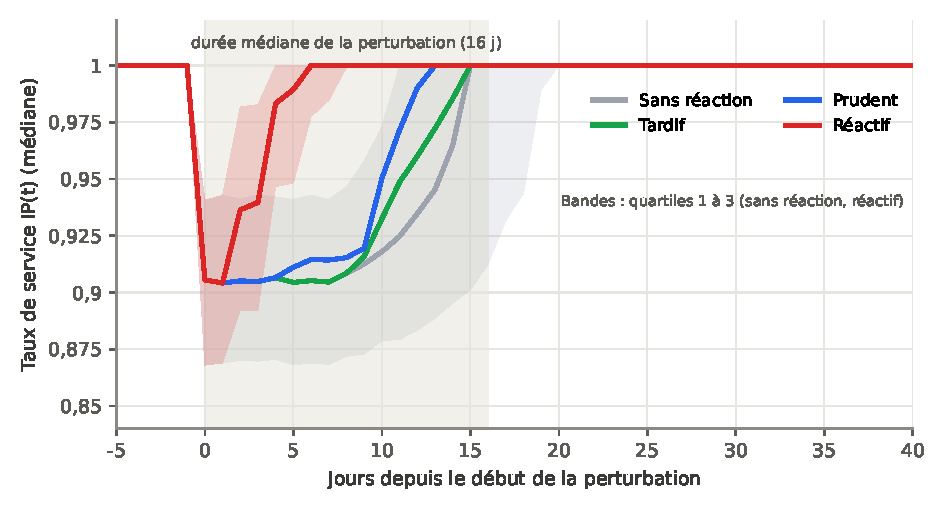
\includegraphics[width=0.62\textwidth]{figures/Fig5_trajectoire_mediane.pdf}
\captionof{figure}{Trajectoire médiane du taux de service selon la politique de gestion (2 000 crises recalées sur le début de la perturbation).}\label{fig:d5}
\end{center}

L'efficacité des politiques dépend de la nature du choc : le profil prudent est sans effet sur une panne fournisseur mais réduit de 41~\% la perte d'une congestion (\voirSM{S5.2}). En classant la perte en trois niveaux de même effectif, le profil prudent atteint le même niveau que le profil réactif dans 18~\% des crises, et cette proportion atteint 31~\% pour les perturbations de 12 jours au plus contre 11~\% au-delà de 18 jours : une crise courte peut être gérée sobrement, une crise longue exige de la réactivité.

Un lot de contrôle de 500 scénarios sur le réseau paramétrique confirme ces proportions : la part du service perdu évitée y atteint 67~\%, 17~\% et 13~\% pour les profils réactif, prudent et tardif. La topologie modifie en revanche l'efficacité des leviers : sur ce réseau aux voies de secours étroites, le profil réactif ne réduit plus que de 25~\% la perte d'une coupure de lien et de 53~\% celle d'une fermeture, contre 73~\% et 82~\% sur ISOMORPH.

\subsection{Pronostic, diagnostic et préconisation}
\label{sec:4.3}

La structure apprise (Fig.~\ref{fig:d6}) compte 41 arcs, sans aucun arc contraire à l'ordre des paliers, et retrouve le mécanisme précédent : la perte cumulée dépend directement de la politique, de la profondeur $h$ et de la durée $d$ du palier, et cette durée dépend de la politique, de la durée de la perturbation et du délai de réaction.

\begin{center}
\resizebox{0.85\textwidth}{!}{% Figure : réseau bayésien appris sous contraintes, avec la distribution marginale de chaque variable
% (données : fichier .bif exporté par BayesArtist ; marginales obtenues par inférence exacte sans observation)
\begin{tikzpicture}[
  bx/.style={draw=#1, fill=#1!10, rounded corners=3pt, minimum width=3.25cm, inner sep=0pt},
  tt/.style={font=\scriptsize\bfseries, text=black!80, anchor=north, align=center, inner sep=1pt},
  ml/.style={font=\tiny, anchor=west, inner sep=0pt},
  pc/.style={font=\tiny, anchor=east, inner sep=0pt},
  a/.style={-{Stealth[length=1.4mm]}, black!30, thin},
  m/.style={-{Stealth[length=2mm]}, polreac, very thick}]
  \node[font=\small\bfseries, text=black!70] at (0.00,6.56) {Contexte};
  % cible
  \node[bx=palctx, minimum height=1.360cm] (cible) at (0.00,3.945) {};
  \node[tt] at (0.00,4.585) {Position de la cible};
  \node[ml] at (-1.53,4.060) {Passage obligé};
  \fill[black!8] (0.095,3.975) rectangle (0.815,4.145);
  \fill[palctx] (0.095,3.975) rectangle (0.137,4.145);
  \node[pc] at (1.54,4.060) {5,8\,\%};
  \node[ml] at (-1.53,3.770) {Site redondé};
  \fill[black!8] (0.095,3.685) rectangle (0.815,3.855);
  \fill[palctx] (0.095,3.685) rectangle (0.488,3.855);
  \node[pc] at (1.54,3.770) {54,6\,\%};
  \node[ml] at (-1.53,3.480) {Réseau entier};
  \fill[black!8] (0.095,3.395) rectangle (0.815,3.565);
  \fill[palctx] (0.095,3.395) rectangle (0.380,3.565);
  \node[pc] at (1.54,3.480) {39,6\,\%};
  % partcrit
  \node[bx=palctx, minimum height=1.630cm] (partcrit) at (0.00,2.050) {};
  \node[tt] at (0.00,2.825) {Part des articles\\critiques};
  \node[ml] at (-1.53,2.030) {Faible};
  \fill[black!8] (0.095,1.945) rectangle (0.815,2.115);
  \fill[palctx] (0.095,1.945) rectangle (0.335,2.115);
  \node[pc] at (1.54,2.030) {33,4\,\%};
  \node[ml] at (-1.53,1.740) {Moyen};
  \fill[black!8] (0.095,1.655) rectangle (0.815,1.825);
  \fill[palctx] (0.095,1.655) rectangle (0.335,1.825);
  \node[pc] at (1.54,1.740) {33,4\,\%};
  \node[ml] at (-1.53,1.450) {Fort};
  \fill[black!8] (0.095,1.365) rectangle (0.815,1.535);
  \fill[palctx] (0.095,1.365) rectangle (0.334,1.535);
  \node[pc] at (1.54,1.450) {33,2\,\%};
  % nature
  \node[bx=palctx, minimum height=1.940cm] (nature) at (0.00,-0.135) {};
  \node[tt] at (0.00,0.795) {Nature};
  \node[ml] at (-1.53,0.270) {Panne fourn.};
  \fill[black!8] (0.095,0.185) rectangle (0.815,0.355);
  \fill[palctx] (0.095,0.185) rectangle (0.250,0.355);
  \node[pc] at (1.54,0.270) {21,5\,\%};
  \node[ml] at (-1.53,-0.020) {Coupure lien};
  \fill[black!8] (0.095,-0.105) rectangle (0.815,0.065);
  \fill[palctx] (0.095,-0.105) rectangle (0.233,0.065);
  \node[pc] at (1.54,-0.020) {19,1\,\%};
  \node[ml] at (-1.53,-0.310) {Fermeture site};
  \fill[black!8] (0.095,-0.395) rectangle (0.815,-0.225);
  \fill[palctx] (0.095,-0.395) rectangle (0.238,-0.225);
  \node[pc] at (1.54,-0.310) {19,8\,\%};
  \node[ml] at (-1.53,-0.600) {Pic demande};
  \fill[black!8] (0.095,-0.685) rectangle (0.815,-0.515);
  \fill[palctx] (0.095,-0.685) rectangle (0.241,-0.515);
  \node[pc] at (1.54,-0.600) {20,3\,\%};
  \node[ml] at (-1.53,-0.890) {Congestion};
  \fill[black!8] (0.095,-0.975) rectangle (0.815,-0.805);
  \fill[palctx] (0.095,-0.975) rectangle (0.235,-0.805);
  \node[pc] at (1.54,-0.890) {19,4\,\%};
  % severite
  \node[bx=palctx, minimum height=1.360cm] (severite) at (0.00,-2.185) {};
  \node[tt] at (0.00,-1.545) {Sévérité};
  \node[ml] at (-1.53,-2.070) {Faible};
  \fill[black!8] (0.095,-2.155) rectangle (0.815,-1.985);
  \fill[palctx] (0.095,-2.155) rectangle (0.335,-1.985);
  \node[pc] at (1.54,-2.070) {33,4\,\%};
  \node[ml] at (-1.53,-2.360) {Moyen};
  \fill[black!8] (0.095,-2.445) rectangle (0.815,-2.275);
  \fill[palctx] (0.095,-2.445) rectangle (0.335,-2.275);
  \node[pc] at (1.54,-2.360) {33,4\,\%};
  \node[ml] at (-1.53,-2.650) {Fort};
  \fill[black!8] (0.095,-2.735) rectangle (0.815,-2.565);
  \fill[palctx] (0.095,-2.735) rectangle (0.334,-2.565);
  \node[pc] at (1.54,-2.650) {33,2\,\%};
  % duree
  \node[bx=palctx, minimum height=1.360cm] (duree) at (0.00,-3.945) {};
  \node[tt] at (0.00,-3.305) {Durée};
  \node[ml] at (-1.53,-3.830) {Faible};
  \fill[black!8] (0.095,-3.915) rectangle (0.815,-3.745);
  \fill[palctx] (0.095,-3.915) rectangle (0.346,-3.745);
  \node[pc] at (1.54,-3.830) {34,8\,\%};
  \node[ml] at (-1.53,-4.120) {Moyen};
  \fill[black!8] (0.095,-4.205) rectangle (0.815,-4.035);
  \fill[palctx] (0.095,-4.205) rectangle (0.328,-4.035);
  \node[pc] at (1.54,-4.120) {32,3\,\%};
  \node[ml] at (-1.53,-4.410) {Fort};
  \fill[black!8] (0.095,-4.495) rectangle (0.815,-4.325);
  \fill[palctx] (0.095,-4.495) rectangle (0.332,-4.325);
  \node[pc] at (1.54,-4.410) {32,9\,\%};
  \node[font=\small\bfseries, text=black!70] at (4.00,6.56) {Politique};
  % profil
  \node[bx=palpol, minimum height=1.650cm] (profil) at (4.00,0.000) {};
  \node[tt] at (4.00,0.785) {Profil de gestion};
  \node[ml] at (2.46,0.260) {Sans réaction};
  \fill[black!8] (4.095,0.175) rectangle (4.815,0.345);
  \fill[palpol] (4.095,0.175) rectangle (4.275,0.345);
  \node[pc] at (5.54,0.260) {25,0\,\%};
  \node[ml] at (2.46,-0.030) {Réactif};
  \fill[black!8] (4.095,-0.115) rectangle (4.815,0.055);
  \fill[palpol] (4.095,-0.115) rectangle (4.275,0.055);
  \node[pc] at (5.54,-0.030) {25,0\,\%};
  \node[ml] at (2.46,-0.320) {Prudent};
  \fill[black!8] (4.095,-0.405) rectangle (4.815,-0.235);
  \fill[palpol] (4.095,-0.405) rectangle (4.275,-0.235);
  \node[pc] at (5.54,-0.320) {25,0\,\%};
  \node[ml] at (2.46,-0.610) {Tardif};
  \fill[black!8] (4.095,-0.695) rectangle (4.815,-0.525);
  \fill[palpol] (4.095,-0.695) rectangle (4.275,-0.525);
  \node[pc] at (5.54,-0.610) {25,0\,\%};
  \node[font=\small\bfseries, text=black!70] at (8.00,6.56) {Réponse};
  % detection
  \node[bx=palrep, minimum height=1.940cm] (detection) at (8.00,4.990) {};
  \node[tt] at (8.00,5.920) {Détection};
  \node[ml] at (6.46,5.395) {J0};
  \fill[black!8] (8.095,5.310) rectangle (8.815,5.480);
  \fill[palrep] (8.095,5.310) rectangle (8.262,5.480);
  \node[pc] at (9.54,5.395) {23,2\,\%};
  \node[ml] at (6.46,5.105) {J1 à J2};
  \fill[black!8] (8.095,5.020) rectangle (8.815,5.190);
  \fill[palrep] (8.095,5.020) rectangle (8.243,5.190);
  \node[pc] at (9.54,5.105) {20,6\,\%};
  \node[ml] at (6.46,4.815) {J3 et plus};
  \fill[black!8] (8.095,4.730) rectangle (8.815,4.900);
  \fill[palrep] (8.095,4.730) rectangle (8.216,4.900);
  \node[pc] at (9.54,4.815) {16,8\,\%};
  \node[ml] at (6.46,4.525) {Non détectée};
  \fill[black!8] (8.095,4.440) rectangle (8.815,4.610);
  \fill[palrep] (8.095,4.440) rectangle (8.199,4.610);
  \node[pc] at (9.54,4.525) {14,4\,\%};
  \node[ml] at (6.46,4.235) {Sans objet};
  \fill[black!8] (8.095,4.150) rectangle (8.815,4.320);
  \fill[palrep] (8.095,4.150) rectangle (8.275,4.320);
  \node[pc] at (9.54,4.235) {25,0\,\%};
  % nbleviers
  \node[bx=palrep, minimum height=1.650cm] (nbleviers) at (8.00,2.795) {};
  \node[tt] at (8.00,3.580) {Nombre de leviers};
  \node[ml] at (6.46,3.055) {0};
  \fill[black!8] (8.095,2.970) rectangle (8.815,3.140);
  \fill[palrep] (8.095,2.970) rectangle (8.377,3.140);
  \node[pc] at (9.54,3.055) {39,2\,\%};
  \node[ml] at (6.46,2.765) {1};
  \fill[black!8] (8.095,2.680) rectangle (8.815,2.850);
  \fill[palrep] (8.095,2.680) rectangle (8.213,2.850);
  \node[pc] at (9.54,2.765) {16,4\,\%};
  \node[ml] at (6.46,2.475) {2};
  \fill[black!8] (8.095,2.390) rectangle (8.815,2.560);
  \fill[palrep] (8.095,2.390) rectangle (8.263,2.560);
  \node[pc] at (9.54,2.475) {23,3\,\%};
  \node[ml] at (6.46,2.185) {3 et plus};
  \fill[black!8] (8.095,2.100) rectangle (8.815,2.270);
  \fill[palrep] (8.095,2.100) rectangle (8.248,2.270);
  \node[pc] at (9.54,2.185) {21,2\,\%};
  % lag
  \node[bx=palrep, minimum height=1.650cm] (lag) at (8.00,0.745) {};
  \node[tt] at (8.00,1.530) {Délai de réaction};
  \node[ml] at (6.46,1.005) {Court};
  \fill[black!8] (8.095,0.920) rectangle (8.815,1.090);
  \fill[palrep] (8.095,0.920) rectangle (8.257,1.090);
  \node[pc] at (9.54,1.005) {22,5\,\%};
  \node[ml] at (6.46,0.715) {Moyen};
  \fill[black!8] (8.095,0.630) rectangle (8.815,0.800);
  \fill[palrep] (8.095,0.630) rectangle (8.278,0.800);
  \node[pc] at (9.54,0.715) {25,4\,\%};
  \node[ml] at (6.46,0.425) {Long};
  \fill[black!8] (8.095,0.340) rectangle (8.815,0.510);
  \fill[palrep] (8.095,0.340) rectangle (8.187,0.510);
  \node[pc] at (9.54,0.425) {12,8\,\%};
  \node[ml] at (6.46,0.135) {Sans objet};
  \fill[black!8] (8.095,0.050) rectangle (8.815,0.220);
  \fill[palrep] (8.095,0.050) rectangle (8.377,0.220);
  \node[pc] at (9.54,0.135) {39,2\,\%};
  % fstock
  \node[bx=palrep, minimum height=1.070cm] (fstock) at (8.00,-1.015) {};
  \node[tt] at (8.00,-0.520) {Leviers de stock};
  \node[ml] at (6.46,-1.045) {Non};
  \fill[black!8] (8.095,-1.130) rectangle (8.815,-0.960);
  \fill[palrep] (8.095,-1.130) rectangle (8.641,-0.960);
  \node[pc] at (9.54,-1.045) {75,8\,\%};
  \node[ml] at (6.46,-1.335) {Oui};
  \fill[black!8] (8.095,-1.420) rectangle (8.815,-1.250);
  \fill[palrep] (8.095,-1.420) rectangle (8.269,-1.250);
  \node[pc] at (9.54,-1.335) {24,2\,\%};
  % freroutage
  \node[bx=palrep, minimum height=1.070cm] (freroutage) at (8.00,-2.485) {};
  \node[tt] at (8.00,-1.990) {Leviers de reroutage};
  \node[ml] at (6.46,-2.515) {Non};
  \fill[black!8] (8.095,-2.600) rectangle (8.815,-2.430);
  \fill[palrep] (8.095,-2.600) rectangle (8.650,-2.430);
  \node[pc] at (9.54,-2.515) {77,1\,\%};
  \node[ml] at (6.46,-2.805) {Oui};
  \fill[black!8] (8.095,-2.890) rectangle (8.815,-2.720);
  \fill[palrep] (8.095,-2.890) rectangle (8.260,-2.720);
  \node[pc] at (9.54,-2.805) {22,9\,\%};
  % fcapacite
  \node[bx=palrep, minimum height=1.070cm] (fcapacite) at (8.00,-3.955) {};
  \node[tt] at (8.00,-3.460) {Leviers de capacité};
  \node[ml] at (6.46,-3.985) {Non};
  \fill[black!8] (8.095,-4.070) rectangle (8.815,-3.900);
  \fill[palrep] (8.095,-4.070) rectangle (8.586,-3.900);
  \node[pc] at (9.54,-3.985) {68,2\,\%};
  \node[ml] at (6.46,-4.275) {Oui};
  \fill[black!8] (8.095,-4.360) rectangle (8.815,-4.190);
  \fill[palrep] (8.095,-4.360) rectangle (8.324,-4.190);
  \node[pc] at (9.54,-4.275) {31,8\,\%};
  % fdemande
  \node[bx=palrep, minimum height=1.070cm] (fdemande) at (8.00,-5.425) {};
  \node[tt] at (8.00,-4.930) {Leviers de demande};
  \node[ml] at (6.46,-5.455) {Non};
  \fill[black!8] (8.095,-5.540) rectangle (8.815,-5.370);
  \fill[palrep] (8.095,-5.540) rectangle (8.628,-5.370);
  \node[pc] at (9.54,-5.455) {74,0\,\%};
  \node[ml] at (6.46,-5.745) {Oui};
  \fill[black!8] (8.095,-5.830) rectangle (8.815,-5.660);
  \fill[palrep] (8.095,-5.830) rectangle (8.282,-5.660);
  \node[pc] at (9.54,-5.745) {26,0\,\%};
  \node[font=\small\bfseries, text=black!70] at (12.00,6.56) {Mécanisme};
  % beta
  \node[bx=palmec, minimum height=1.360cm] (beta) at (12.00,2.640) {};
  \node[tt] at (12.00,3.280) {$\beta$ (reprise)};
  \node[ml] at (10.46,2.755) {Faible};
  \fill[black!8] (12.095,2.670) rectangle (12.815,2.840);
  \fill[palmec] (12.095,2.670) rectangle (12.337,2.840);
  \node[pc] at (13.54,2.755) {33,6\,\%};
  \node[ml] at (10.46,2.465) {Moyen};
  \fill[black!8] (12.095,2.380) rectangle (12.815,2.550);
  \fill[palmec] (12.095,2.380) rectangle (12.331,2.550);
  \node[pc] at (13.54,2.465) {32,8\,\%};
  \node[ml] at (10.46,2.175) {Fort};
  \fill[black!8] (12.095,2.090) rectangle (12.815,2.260);
  \fill[palmec] (12.095,2.090) rectangle (12.337,2.260);
  \node[pc] at (13.54,2.175) {33,6\,\%};
  % h
  \node[bx=palmec, minimum height=1.360cm] (h) at (12.00,0.880) {};
  \node[tt] at (12.00,1.520) {$h$ (profondeur)};
  \node[ml] at (10.46,0.995) {Faible};
  \fill[black!8] (12.095,0.910) rectangle (12.815,1.080);
  \fill[palmec] (12.095,0.910) rectangle (12.338,1.080);
  \node[pc] at (13.54,0.995) {33,7\,\%};
  \node[ml] at (10.46,0.705) {Moyen};
  \fill[black!8] (12.095,0.620) rectangle (12.815,0.790);
  \fill[palmec] (12.095,0.620) rectangle (12.335,0.790);
  \node[pc] at (13.54,0.705) {33,4\,\%};
  \node[ml] at (10.46,0.415) {Fort};
  \fill[black!8] (12.095,0.330) rectangle (12.815,0.500);
  \fill[palmec] (12.095,0.330) rectangle (12.331,0.500);
  \node[pc] at (13.54,0.415) {32,8\,\%};
  % alpha
  \node[bx=palmec, minimum height=1.360cm] (alpha) at (12.00,-0.880) {};
  \node[tt] at (12.00,-0.240) {$\alpha$ (chute)};
  \node[ml] at (10.46,-0.765) {Faible};
  \fill[black!8] (12.095,-0.850) rectangle (12.815,-0.680);
  \fill[palmec] (12.095,-0.850) rectangle (12.334,-0.680);
  \node[pc] at (13.54,-0.765) {33,2\,\%};
  \node[ml] at (10.46,-1.055) {Moyen};
  \fill[black!8] (12.095,-1.140) rectangle (12.815,-0.970);
  \fill[palmec] (12.095,-1.140) rectangle (12.335,-0.970);
  \node[pc] at (13.54,-1.055) {33,3\,\%};
  \node[ml] at (10.46,-1.345) {Fort};
  \fill[black!8] (12.095,-1.430) rectangle (12.815,-1.260);
  \fill[palmec] (12.095,-1.430) rectangle (12.335,-1.260);
  \node[pc] at (13.54,-1.345) {33,4\,\%};
  % d
  \node[bx=palmec, minimum height=1.360cm] (d) at (12.00,-2.640) {};
  \node[tt] at (12.00,-2.000) {$d$ (durée du palier)};
  \node[ml] at (10.46,-2.525) {Faible};
  \fill[black!8] (12.095,-2.610) rectangle (12.815,-2.440);
  \fill[palmec] (12.095,-2.610) rectangle (12.338,-2.440);
  \node[pc] at (13.54,-2.525) {33,8\,\%};
  \node[ml] at (10.46,-2.815) {Moyen};
  \fill[black!8] (12.095,-2.900) rectangle (12.815,-2.730);
  \fill[palmec] (12.095,-2.900) rectangle (12.334,-2.730);
  \node[pc] at (13.54,-2.815) {33,2\,\%};
  \node[ml] at (10.46,-3.105) {Fort};
  \fill[black!8] (12.095,-3.190) rectangle (12.815,-3.020);
  \fill[palmec] (12.095,-3.190) rectangle (12.333,-3.020);
  \node[pc] at (13.54,-3.105) {33,0\,\%};
  \node[font=\small\bfseries, text=black!70] at (16.00,6.56) {Résilience};
  % CRD
  \node[bx=palres, minimum height=1.360cm] (CRD) at (16.00,1.760) {};
  \node[tt] at (16.00,2.400) {CRD};
  \node[ml] at (14.46,1.875) {Faible};
  \fill[black!8] (16.095,1.790) rectangle (16.815,1.960);
  \fill[palres] (16.095,1.790) rectangle (16.345,1.960);
  \node[pc] at (17.55,1.875) {34,7\,\%};
  \node[ml] at (14.46,1.585) {Moyen};
  \fill[black!8] (16.095,1.500) rectangle (16.815,1.670);
  \fill[palres] (16.095,1.500) rectangle (16.320,1.670);
  \node[pc] at (17.55,1.585) {31,3\,\%};
  \node[ml] at (14.46,1.295) {Fort};
  \fill[black!8] (16.095,1.210) rectangle (16.815,1.380);
  \fill[palres] (16.095,1.210) rectangle (16.340,1.380);
  \node[pc] at (17.55,1.295) {34,0\,\%};
  % IPC
  \node[bx=palres, minimum height=1.360cm] (IPC) at (16.00,0.000) {};
  \node[tt] at (16.00,0.640) {IPC};
  \node[ml] at (14.46,0.115) {Faible};
  \fill[black!8] (16.095,0.030) rectangle (16.815,0.200);
  \fill[palres] (16.095,0.030) rectangle (16.341,0.200);
  \node[pc] at (17.55,0.115) {34,1\,\%};
  \node[ml] at (14.46,-0.175) {Moyen};
  \fill[black!8] (16.095,-0.260) rectangle (16.815,-0.090);
  \fill[palres] (16.095,-0.260) rectangle (16.333,-0.090);
  \node[pc] at (17.55,-0.175) {33,0\,\%};
  \node[ml] at (14.46,-0.465) {Fort};
  \fill[black!8] (16.095,-0.550) rectangle (16.815,-0.380);
  \fill[palres] (16.095,-0.550) rectangle (16.332,-0.380);
  \node[pc] at (17.55,-0.465) {32,9\,\%};
  % TRP
  \node[bx=palres, minimum height=1.360cm] (TRP) at (16.00,-1.760) {};
  \node[tt] at (16.00,-1.120) {TRP};
  \node[ml] at (14.46,-1.645) {Faible};
  \fill[black!8] (16.095,-1.730) rectangle (16.815,-1.560);
  \fill[palres] (16.095,-1.730) rectangle (16.335,-1.560);
  \node[pc] at (17.55,-1.645) {33,3\,\%};
  \node[ml] at (14.46,-1.935) {Moyen};
  \fill[black!8] (16.095,-2.020) rectangle (16.815,-1.850);
  \fill[palres] (16.095,-2.020) rectangle (16.344,-1.850);
  \node[pc] at (17.55,-1.935) {34,6\,\%};
  \node[ml] at (14.46,-2.225) {Fort};
  \fill[black!8] (16.095,-2.310) rectangle (16.815,-2.140);
  \fill[palres] (16.095,-2.310) rectangle (16.326,-2.140);
  \node[pc] at (17.55,-2.225) {32,1\,\%};
  \begin{scope}[on background layer]
    \draw[a] (cible.west) to[bend right=26] (nature.west);
    \draw[a] (cible.east) -- (detection.west);
    \draw[a] (profil.east) -- (detection.west);
    \draw[a] (nature.west) to[bend right=26] (severite.west);
    \draw[a] (nature.east) -- (nbleviers.west);
    \draw[a] (detection.east) to[bend left=26] (nbleviers.east);
    \draw[a] (severite.west) to[bend right=26] (duree.west);
    \draw[a] (profil.east) -- (beta.west);
    \draw[a] (nbleviers.east) -- (beta.west);
    \draw[a] (nature.east) -- (freroutage.west);
    \draw[a] (profil.east) -- (freroutage.west);
    \draw[a] (nbleviers.east) to[bend left=26] (freroutage.east);
    \draw[a] (nature.east) -- (fdemande.west);
    \draw[a] (profil.east) -- (fdemande.west);
    \draw[a] (nbleviers.east) to[bend left=26] (fdemande.east);
    \draw[a] (beta.east) to[bend left=26] (h.east);
    \draw[a] (detection.east) -- (h.west);
    \draw[a] (fdemande.east) -- (h.west);
    \draw[a] (profil.east) -- (fstock.west);
    \draw[a] (nbleviers.east) to[bend left=26] (fstock.east);
    \draw[a] (freroutage.east) to[bend right=26] (fstock.east);
    \draw[a] (h.east) to[bend left=26] (alpha.east);
    \draw[a] (beta.east) to[bend left=26] (alpha.east);
    \draw[a] (detection.east) to[bend left=26] (lag.east);
    \draw[a] (nbleviers.east) to[bend left=26] (lag.east);
    \draw[a] (fstock.east) to[bend right=26] (lag.east);
    \draw[a] (nature.east) -- (fcapacite.west);
    \draw[a] (nbleviers.east) to[bend left=26] (fcapacite.east);
    \draw[a] (fstock.east) to[bend left=26] (fcapacite.east);
    \draw[m] (profil.east) -- (d.west);
    \draw[m] (duree.east) -- (d.west);
    \draw[m] (lag.east) -- (d.west);
    \draw[m] (profil.east) -- (IPC.west);
    \draw[m] (h.east) -- (IPC.west);
    \draw[m] (d.east) -- (IPC.west);
    \draw[a] (d.east) -- (CRD.west);
    \draw[a] (alpha.east) -- (CRD.west);
    \draw[a] (beta.east) -- (CRD.west);
    \draw[a] (duree.east) -- (TRP.west);
    \draw[a] (d.east) -- (TRP.west);
    \draw[a] (CRD.east) to[bend left=26] (TRP.east);
  \end{scope}
  \node[font=\scriptsize, text=black!65, anchor=north, text width=17cm, align=center] at (8.00,-6.21) {Trait épais : chemin principal (la politique agit sur la durée $d$ du palier dégradé, qui détermine la perte cumulée IPC). 20 variables, 41 arcs. Barres : probabilité marginale de chaque modalité.};
\end{tikzpicture}

% ANCIEN TIKZ (structure seule, sans les modalités), conservé en commentaire
% % Figure : réseau bayésien appris sous contraintes (données : fichier .bif exporté par BayesArtist)
% \begin{tikzpicture}[x=1.18cm,y=0.98cm,
%   n/.style={draw=#1, fill=#1!12, rounded corners=3pt, font=\scriptsize, align=center, minimum width=1.9cm, minimum height=0.72cm, inner sep=1.2pt},
%   a/.style={-{Stealth[length=1.4mm]}, black!30, thin},
%   m/.style={-{Stealth[length=2mm]}, polreac, very thick}]
%   \node[font=\small\bfseries, text=black!70] at (0,5.6) {Contexte};
%   \node[n=palctx] (cible) at (0,2.700) {Position\\de la cible};
%   \node[n=palctx] (partcrit) at (0,1.350) {Part des articles\\critiques};
%   \node[n=palctx] (nature) at (0,0.000) {Nature};
%   \node[n=palctx] (severite) at (0,-1.350) {Sévérité};
%   \node[n=palctx] (duree) at (0,-2.700) {Durée};
%   \node[font=\small\bfseries, text=black!70] at (2.9,5.6) {Politique};
%   \node[n=palpol] (profil) at (2.9,0.000) {Profil de\\gestion};
%   \node[font=\small\bfseries, text=black!70] at (5.8,5.6) {Réponse};
%   \node[n=palrep] (detection) at (5.8,4.050) {Détection};
%   \node[n=palrep] (nbleviers) at (5.8,2.700) {Nombre\\de leviers};
%   \node[n=palrep] (lag) at (5.8,1.350) {Délai de\\réaction};
%   \node[n=palrep] (fstock) at (5.8,0.000) {Leviers\\de stock};
%   \node[n=palrep] (freroutage) at (5.8,-1.350) {Leviers de\\reroutage};
%   \node[n=palrep] (fcapacite) at (5.8,-2.700) {Leviers de\\capacité};
%   \node[n=palrep] (fdemande) at (5.8,-4.050) {Leviers\\de demande};
%   \node[font=\small\bfseries, text=black!70] at (8.7,5.6) {Mécanisme};
%   \node[n=palmec] (beta) at (8.7,2.025) {$\beta$ (reprise)};
%   \node[n=palmec] (h) at (8.7,0.675) {$h$ (profondeur)};
%   \node[n=palmec] (alpha) at (8.7,-0.675) {$\alpha$ (chute)};
%   \node[n=palmec] (d) at (8.7,-2.025) {$d$ (durée\\du palier)};
%   \node[font=\small\bfseries, text=black!70] at (11.6,5.6) {Résilience};
%   \node[n=palres] (CRD) at (11.6,1.350) {CRD};
%   \node[n=palres] (IPC) at (11.6,0.000) {IPC};
%   \node[n=palres] (TRP) at (11.6,-1.350) {TRP};
%   \begin{scope}[on background layer]
%     \draw[a] (cible.west) to[bend right=40] (nature.west);
%     \draw[a] (cible.east) -- (detection.west);
%     \draw[a] (profil.east) -- (detection.west);
%     \draw[a] (nature.west) to[bend right=40] (severite.west);
%     \draw[a] (nature.east) -- (nbleviers.west);
%     \draw[a] (detection.east) to[bend left=40] (nbleviers.east);
%     \draw[a] (severite.west) to[bend right=40] (duree.west);
%     \draw[a] (profil.east) -- (beta.west);
%     \draw[a] (nbleviers.east) -- (beta.west);
%     \draw[a] (nature.east) -- (freroutage.west);
%     \draw[a] (profil.east) -- (freroutage.west);
%     \draw[a] (nbleviers.east) to[bend left=40] (freroutage.east);
%     \draw[a] (nature.east) -- (fdemande.west);
%     \draw[a] (profil.east) -- (fdemande.west);
%     \draw[a] (nbleviers.east) to[bend left=40] (fdemande.east);
%     \draw[a] (beta.east) to[bend left=40] (h.east);
%     \draw[a] (detection.east) -- (h.west);
%     \draw[a] (fdemande.east) -- (h.west);
%     \draw[a] (profil.east) -- (fstock.west);
%     \draw[a] (nbleviers.east) to[bend left=40] (fstock.east);
%     \draw[a] (freroutage.east) to[bend right=40] (fstock.east);
%     \draw[a] (h.east) to[bend left=40] (alpha.east);
%     \draw[a] (beta.east) to[bend left=40] (alpha.east);
%     \draw[a] (detection.east) to[bend left=40] (lag.east);
%     \draw[a] (nbleviers.east) to[bend left=40] (lag.east);
%     \draw[a] (fstock.east) to[bend right=40] (lag.east);
%     \draw[a] (nature.east) -- (fcapacite.west);
%     \draw[a] (nbleviers.east) to[bend left=40] (fcapacite.east);
%     \draw[a] (fstock.east) to[bend left=40] (fcapacite.east);
%     \draw[m] (profil.east) -- (d.west);
%     \draw[m] (duree.east) -- (d.west);
%     \draw[m] (lag.east) -- (d.west);
%     \draw[m] (profil.east) -- (IPC.west);
%     \draw[m] (h.east) -- (IPC.west);
%     \draw[m] (d.east) -- (IPC.west);
%     \draw[a] (d.east) -- (CRD.west);
%     \draw[a] (alpha.east) -- (CRD.west);
%     \draw[a] (beta.east) -- (CRD.west);
%     \draw[a] (duree.east) -- (TRP.west);
%     \draw[a] (d.east) -- (TRP.west);
%     \draw[a] (CRD.east) to[bend left=40] (TRP.east);
%   \end{scope}
%   \node[font=\scriptsize, text=black!65, anchor=north] at (5.8,-5.1) {Trait épais : chemin principal (la politique agit sur la durée $d$ du palier dégradé, qui détermine la perte cumulée IPC). 20 variables, 41 arcs.};
% \end{tikzpicture}
}
\captionof{figure}{Réseau bayésien appris sous contraintes, variables colorées par palier de l'ordre temporel d'une crise.}\label{fig:d6}
\end{center}

Le pronostic, établi à partir des seules variables connues au moment de décider, classe correctement 65~\% des crises de test, contre 34~\% pour la classe majoritaire et 60~\% pour un modèle fondé sur la seule politique (score de Brier de 0,466 contre 0,667 et 0,494). La courbe d'apprentissage est presque plate : la limite tient à l'information disponible au moment de décider, non à la taille de la base. Le diagnostic est bien calibré pour la politique et la durée : pour les crises de test à forte perte, les probabilités a posteriori des politiques reproduisent leurs fréquences observées à 0,01 près.

Avec l'objectif d'une perte faible, seul le profil réactif réussit régulièrement, et la règle le préconise toujours. Avec l'objectif moins exigeant d'une perte qui ne soit pas forte, un arbitrage apparaît entre sécurité et sobriété, que règle le seuil $\theta$ (tableau~\ref{tab:d15}).

\begin{table*}[htbp]
\caption{Préconisation sur les crises de test, objectif d'une perte cumulée non forte.}
\label{tab:d15}
\footnotesize
\begin{tabularx}{\textwidth}{@{}LLL@{}}
\toprule
\textbf{Règle} & \textbf{Objectif atteint} & \textbf{Préconisations plus sobres que le profil réactif} \\
\midrule
Toujours le profil réactif & 99,2 \% & 0 \% \\
Réseau appris, $\theta$ = 0,9 & 99,2 \% & 0 \% \\
Réseau appris, $\theta$ = 0,8 & 97,5 \% & 15 \% \\
Réseau appris, $\theta$ = 0,7 & 86,2 \% & 37 \% \\
Réseau appris, $\theta$ = 0,6 & 69,5 \% & 84 \% \\
Référence a posteriori : politique la plus sobre ayant réussi & 99,2 \% & 67 \% \\
\bottomrule
\end{tabularx}
\end{table*}

Avec $\theta$ = 0,8, le réseau préconise une politique plus sobre dans environ une crise sur sept, pour un taux de réussite de 97,5~\%, moins de deux points sous la politique la plus interventionniste. Cette sobriété repose entièrement sur la durée prévue du choc : lorsque cette information est retirée de la description de la crise, la règle ne préconise plus aucune politique sobre. Une estimation de la durée d'une perturbation a donc une valeur décisionnelle propre. Ainsi, pour la fermeture courte d'un site redondé, le profil prudent atteint l'objectif avec une probabilité de 0,80 et devient la préconisation, alors que pour la fermeture longue d'un point de passage obligé seul le profil réactif y parvient (\voirSM{S5.3}).

La figure~\ref{fig:carte} généralise cette lecture par l'inférence à rebours, pour l'objectif d'une perte faible, aux sept contextes que la topologie d'ISOMORPH rend possibles. Le profil réactif est le plus probable partout, et d'autant plus que le choc dure : sa probabilité a posteriori passe de 0,51 à 0,58 pour un choc court à 0,72 à 0,79 pour un choc long. Pour un choc court, les autres politiques conservent chacune entre 0,12 et 0,18 : une perte faible y reste accessible sans réaction rapide.

\begin{center}
\begin{minipage}{\textwidth}\centering
% Figure : carte de préconisation par inférence à rebours sur le réseau appris, en nuage de points.
% Probabilité a posteriori de chaque profil sachant IPC = faible, pour les sept contextes (nature, position de la cible),
% un plan par durée du choc. Vert : politique la plus probable du contexte ; rouge : autres politiques.
% Valeurs identiques à l'ancienne carte (inférence exacte sur le réseau appris, fichier .bif).
\begin{tikzpicture}
\pgfplotsset{carte/.style={width=5.6cm, height=5.6cm, xmin=0.5, xmax=4.5, ymin=0, ymax=0.85,
  xtick={1,2,3,4}, xticklabels={Aucune,Tardif,Prudent,Réactif},
  ytick={0,0.2,0.4,0.6,0.8}, yticklabel style={/pgf/number format/.cd,fixed,fixed zerofill,precision=1,use comma},
  tick label style={font=\scriptsize}, label style={font=\scriptsize}, title style={font=\small\bfseries},
  ymajorgrids, grid style={gray!20}, axis lines*=left, clip=false}}
\begin{axis}[carte, title={Durée courte}, at={(0.0cm,0)}, ylabel={Probabilité a posteriori du profil}]
  \addplot[only marks, mark=*, mark size=1.8pt, appreac, fill opacity=0.75, draw opacity=0.9] coordinates {(0.73,0.16) (1.73,0.15) (2.73,0.12) (0.82,0.15) (1.82,0.14) (2.82,0.13) (0.91,0.13) (1.91,0.18) (2.91,0.17) (1.00,0.14) (2.00,0.18) (3.00,0.17) (1.09,0.14) (2.09,0.17) (3.09,0.17) (1.18,0.15) (2.18,0.15) (3.18,0.15) (1.27,0.15) (2.27,0.15) (3.27,0.15)};
  \addplot[only marks, mark=*, mark size=1.8pt, apptard, fill opacity=0.85] coordinates {(3.73,0.58) (3.82,0.57) (3.91,0.52) (4.00,0.51) (4.09,0.52) (4.18,0.55) (4.27,0.55)};
\end{axis}
\begin{axis}[carte, title={Durée moyenne}, at={(5.15cm,0)}, yticklabels={}]
  \addplot[only marks, mark=*, mark size=1.8pt, appreac, fill opacity=0.75, draw opacity=0.9] coordinates {(0.73,0.07) (1.73,0.07) (2.73,0.10) (0.82,0.06) (1.82,0.07) (2.82,0.12) (0.91,0.06) (1.91,0.10) (2.91,0.14) (1.00,0.06) (2.00,0.10) (3.00,0.14) (1.09,0.06) (2.09,0.10) (3.09,0.14) (1.18,0.07) (2.18,0.08) (3.18,0.12) (1.27,0.07) (2.27,0.08) (3.27,0.12)};
  \addplot[only marks, mark=*, mark size=1.8pt, apptard, fill opacity=0.85] coordinates {(3.73,0.76) (3.82,0.75) (3.91,0.69) (4.00,0.70) (4.09,0.70) (4.18,0.73) (4.27,0.73)};
\end{axis}
\begin{axis}[carte, title={Durée longue}, at={(10.3cm,0)}, yticklabels={}]
  \addplot[only marks, mark=*, mark size=1.8pt, appreac, fill opacity=0.75, draw opacity=0.9] coordinates {(0.73,0.06) (1.73,0.07) (2.73,0.08) (0.82,0.06) (1.82,0.07) (2.82,0.10) (0.91,0.05) (1.91,0.10) (2.91,0.13) (1.00,0.05) (2.00,0.09) (3.00,0.13) (1.09,0.05) (2.09,0.09) (3.09,0.13) (1.18,0.06) (2.18,0.08) (3.18,0.10) (1.27,0.06) (2.27,0.08) (3.27,0.10)};
  \addplot[only marks, mark=*, mark size=1.8pt, apptard, fill opacity=0.85] coordinates {(3.73,0.79) (3.82,0.77) (3.91,0.72) (4.00,0.72) (4.09,0.73) (4.18,0.76) (4.27,0.76)};
\end{axis}
\matrix[anchor=north, font=\scriptsize, column sep=4pt] at (7.6cm,-0.5cm) {
  \fill[apptard] (0,0) circle (2pt); & \node[anchor=west]{Politique la plus probable du contexte}; &
  \fill[appreac] (0,0) circle (2pt); & \node[anchor=west]{Autres politiques}; \\
};
\end{tikzpicture}

\captionof{figure}{Carte de préconisation : probabilité a posteriori de chaque profil sachant une perte cumulée faible, pour les sept contextes de nature et de position de la cible, selon la durée du choc.}\label{fig:carte}
\end{minipage}
\end{center}

\subsection{Rôle des stocks}
\label{sec:4.4}

La représentation temporelle permet d'étudier le rôle des stocks, que la base principale neutralise : 60 crises sans réaction ont été simulées sur ISOMORPH pour chaque nature et chaque couverture de stock. Pour les ruptures de distribution, la couverture agit comme un levier de robustesse progressif : plus elle est faible, plus les crises visibles sont nombreuses, de 11 à 43 sur 60 pour une coupure de lien. Le pic de demande est au contraire mieux absorbé sans stocks, le surcroît de demande devant d'abord être prélevé sur des stocks dimensionnés sur le débit nominal. La couverture de stock n'est donc pas un levier universel de résilience : elle protège contre les pertes de capacité de distribution, mais pas contre un choc de demande (\voirSM{S5.4}).

\subsection{Lecture économique}
\label{sec:4.5}

Multipliée par la demande journalière de référence, la part de service non rendue pendant les 60 jours qui suivent le choc donne les ventes perdues : une crise sans réaction coûte en moyenne 25 550 unités, soit environ 1,4 jour de demande. Le modèle ne valorisant pas les leviers, leur coût $c$ par engagement est exprimé en unités de marge $m$ : une politique est rentable tant que les ventes préservées, multipliées par $m$, couvrent le coût des leviers engagés, et le rapport $c/m$ au-delà duquel ce n'est plus le cas constitue son seuil de rentabilité (tableau~\ref{tab:eco}).

\begin{table*}[htbp]
\caption{Ventes préservées, leviers engagés et seuil de rentabilité par politique (moyennes sur 2 000 crises). Le gain marginal rapporte le surcroît de ventes préservées au surcroît de leviers par rapport à la ligne précédente.}
\label{tab:eco}
\footnotesize
\begin{tabularx}{\textwidth}{@{}LLLLLL@{}}
\toprule
\textbf{Politique} & \textbf{Ventes perdues par crise (unités)} & \textbf{Ventes préservées (unités ; part)} & \textbf{Leviers engagés par crise} & \textbf{Seuil de rentabilité ($c/m$)} & \textbf{Gain marginal par levier} \\
\midrule
Sans réaction & 25 550 & référence & 0 & sans objet & sans objet \\
Tardif & 22 020 & 3 530 ; 14~\% & 0,67 & 5 300 & 5 300 \\
Prudent & 20 980 & 4 570 ; 18~\% & 1,97 & 2 320 & 790 \\
Réactif & 7 000 & 18 550 ; 73~\% & 2,80 & 6 630 & 16 940 \\
\bottomrule
\end{tabularx}
\end{table*}

La politique réactive est à la fois la plus efficace et la plus rentable par levier : chacun de ses leviers préserve en moyenne 6 630 unités, soit environ un tiers de journée de demande. La politique prudente est au contraire économiquement dominée : elle engage plus des deux tiers des leviers de la politique réactive pour un quart de ses gains, et chaque levier qu'elle ajoute à la politique tardive ne préserve que 790 unités. Le coût d'une politique tient donc moins au nombre de leviers qu'à leur moment d'engagement.

\begin{center}
% Figure : bénéfice net moyen d'une politique par crise, selon le coût d'un levier
% (données : ip_timeseries.csv et base d'apprentissage du lot A ; calcul décrit en section 6.6)
\begin{tikzpicture}
\begin{axis}[
  width=0.93\textwidth, height=5.8cm,
  xmin=0, xmax=12000, ymin=-6, ymax=20,
  xlabel={Coût d'un levier engagé, exprimé en unités de marge ($c/m$)},
  ylabel style={align=center},
  ylabel={Bénéfice net moyen par crise\\(milliers d'unités de marge)},
  xtick={0,2000,4000,6000,8000,10000,12000},
  xticklabel style={/pgf/number format/.cd,1000 sep={\,}},
  scaled x ticks=false,
  tick label style={font=\scriptsize}, label style={font=\small},
  grid=major, grid style={black!8},
  legend style={font=\scriptsize, draw=none, fill=white, fill opacity=0.9, text opacity=1, at={(0.98,0.98)}, anchor=north east, cells={anchor=west}},
  every axis plot/.append style={line width=1.2pt}]
  \fill[appreac!6] (axis cs:0,-6) rectangle (axis cs:6628,20);
  \node[font=\scriptsize, text=appreac!85!black, anchor=south west, align=left] at (axis cs:150,-5.6) {zone où la politique\\réactive est rentable};
  \addplot[appnone] table[x=r, y expr=\thisrow{none}/1000] {figures/data/eco_benefice.dat};
  \addlegendentry{Sans réaction}
  \addplot[apptard] table[x=r, y expr=\thisrow{tardif}/1000] {figures/data/eco_benefice.dat};
  \addlegendentry{Tardif}
  \addplot[appprud] table[x=r, y expr=\thisrow{prudent}/1000] {figures/data/eco_benefice.dat};
  \addlegendentry{Prudent}
  \addplot[appreac] table[x=r, y expr=\thisrow{reactif}/1000] {figures/data/eco_benefice.dat};
  \addlegendentry{Réactif}
  \addplot[black!75, line width=1.6pt, densely dashed] table[x=r, y expr=\thisrow{posteriori}/1000] {figures/data/eco_benefice.dat};
  \addlegendentry{Meilleure politique choisie crise par crise}
  \draw[black!50, densely dotted] (axis cs:6628,-6) -- (axis cs:6628,20);
  \node[font=\scriptsize, fill=white, inner sep=1pt, anchor=west] at (axis cs:6750,9.3) {seuil de la politique réactive : 6 630};
\end{axis}
\end{tikzpicture}
\captionof{figure}{Bénéfice net moyen par crise selon le coût d'un levier. La courbe en tirets, qui choisit a posteriori la meilleure politique pour chaque crise, borne la valeur d'une préconisation adaptée.}\label{fig:eco}
\end{center}

Parmi les politiques fixes, la réactivité est optimale tant que le coût d'un levier reste sous 6 630 unités de marge ; au-delà, mieux vaut ne pas réagir (Fig.~\ref{fig:eco}). Choisir pour chaque crise la politique au meilleur bénéfice, comme si son issue était connue d'avance, porterait le bénéfice moyen de 4 560 à 8 350 unités par crise pour un levier de 5 000 unités de marge, soit 83~\% de plus que la meilleure politique fixe. Face à des perturbations mineures, en revanche, le profil réactif engage des leviers près de trente fois moins rentables que sur une crise sévère (\voirSM{S5.5}).

\section{Discussion}
\label{sec:5}

\subsection{Apports théoriques}
\label{sec:5.1}

La première contribution est méthodologique : la démarche produit des données reliant perturbation, décisions et taux de service, avec une propriété que les données d'observation n'ont jamais, chaque crise étant observée sous plusieurs politiques, toutes choses égales par ailleurs. La politique devient ainsi une intervention au sens de \citet{pearl2009}, dont l'effet est identifiable par construction, et une préconisation peut être confrontée à ce qui se serait réellement produit.

La deuxième contribution porte sur la représentation de la résilience. La courbe de perte et de rétablissement \citep{bruneau2003} et le profil de perturbation \citep{sheffi2005book} résument une crise par sa profondeur et sa durée. Les résultats montrent que ces deux dimensions ne relèvent pas des mêmes causes : la profondeur dépend surtout du choc, la durée surtout de la gestion. Décomposer la trajectoire en paramètres de mécanisme est donc la condition pour attribuer une perte à sa cause, et le réseau appris retrouve ce partage sans qu'il lui soit imposé.

La troisième contribution précise la typologie des stratégies de contingence \citep{tomlin2006,chopra2004}. L'efficacité d'un levier n'est pas une propriété du levier, mais de sa rencontre avec la nature du choc et la topologie du réseau : le déstockage est sans effet sur une panne fournisseur mais atténue une congestion, et la réaction la plus rapide perd de son efficacité lorsque les voies de secours sont étroites. Ces interactions plaident pour des règles de pilotage conditionnelles, propres au réseau considéré.

La domination du profil réactif ne rend pas la préconisation triviale : la réactivité n'est ni toujours rentable ni toujours nécessaire, une politique plus sobre suffisant dans deux crises de test sur trois pour éviter une perte forte. L'enjeu est d'arbitrer, crise par crise, entre le coût des leviers et la résilience obtenue.

\subsection{Implications managériales}
\label{sec:5.2}

Il suffit à une entreprise de connaître le rapport entre le coût d'un levier et sa marge unitaire pour situer sa politique sur la figure~\ref{fig:eco}. La vitesse de détection et de décision compte davantage que le nombre de leviers : investir dans la surveillance du taux de service et dans des délégations de décision pré-établies est prioritaire, et moins coûteux que multiplier les leviers. L'information sur la durée prévisible d'un choc a une valeur économique propre, puisqu'elle seule rend possible une politique plus sobre sans perte notable de résilience ; la communication avec fournisseurs et transporteurs sur la durée des incidents mérite d'être organisée avant la crise. Les points de passage obligés réduisent l'efficacité de toute réaction et justifient des investissements de redondance ciblés. Enfin, une réserve d'urgence gagne à être tenue séparée de la politique de commande, faute de quoi elle peut perturber le signal de réapprovisionnement.

\subsection{Limites}
\label{sec:5.3}

Les résultats reposent sur des données simulées. Les valeurs posées faute de données de terrain ont été choisies pour être plausibles et sont toutes réglables, mais elles conditionnent les ordres de grandeur : seules les tendances et les hiérarchies, stables entre les deux réseaux étudiés, doivent être généralisées, et une validation sur des données d'entreprise reste nécessaire. Les leviers n'ont pas de coût et restent engagés jusqu'à la fin de la période observée, ce qui rend la domination de la réactivité en partie structurelle. La nature de la perturbation est supposée diagnostiquée sans erreur, chaque scénario ne comporte qu'une perturbation, les crises touchant un point de passage obligé sont trop rares pour que leurs effets propres soient appris, et l'interaction entre couverture de stock et politique de gestion n'a pas été étudiée.

\section{Conclusion}
\label{sec:6}

Cet article est parti d'une question simple pour un gestionnaire : face à une perturbation, quelle réaction mène au niveau de résilience visé, et après coup, la perte tenait-elle au choc, au réseau ou à la réaction ? Y répondre supposait des crises observées sous plusieurs gestions, ce qu'aucune donnée réelle ne fournit. La démarche proposée les produit par simulation, en rejouant chaque crise à l'identique sous plusieurs politiques, puis les mesure par une courbe de résilience à paramètres interprétables et en apprend un réseau bayésien dont l'effet de la politique est identifiable.

Sur 2 000 crises simulées sur le réseau ISOMORPH, la réaction agit sur la durée d'une crise plutôt que sur sa profondeur, et c'est le moment d'engagement des leviers, plus que leur nombre, qui fait leur rentabilité. Le réseau appris préconise une politique plus sobre dans environ une crise sur sept lorsque la durée du choc est connue, sans perte notable de résilience : l'information sur la durée d'un incident a donc une valeur décisionnelle propre.

Trois prolongements en découlent. Le premier est l'effet de la topologie : à perturbation et décision identiques, deux réseaux réagissent différemment, et le générateur permet d'étudier systématiquement cet effet sur plusieurs topologies, jusqu'à la reconfiguration du réseau elle-même comme levier de résilience. Le deuxième est économique : valoriser le coût des leviers et leur levée transformerait la préconisation en arbitrage explicite entre coût et résilience. Le troisième est empirique : confronter les préconisations à des crises réelles, même partiellement documentées.

% Déclarations finales : disponibilité des données, usage de l'IA générative, intérêts, financement.

\section*{Disponibilité des données}

Les données et le code qui permettent de reproduire les résultats sont déposés dans un entrepôt public, conformément à la politique de données de la revue. Le jeu de données Mendeley Data \citep{screborn2026data} réunit les bases de scénarios des lots A, B et C, les fichiers d'hypothèses et de configuration, les trajectoires, les paramètres ajustés, la base d'apprentissage, les contraintes structurelles et le réseau bayésien appris, ainsi que le générateur Isomorph-Reborn, diffusé en code ouvert avec son manuel d'utilisation. Pendant l'évaluation, il est accessible par un lien de consultation réservé aux relecteurs : \url{https://data.mendeley.com/preview/jm2phpyw92?a=b897008c-f117-4563-85e2-fb74ac173c47}. L'outil BayesArtist, utilisé pour l'apprentissage et l'inférence, n'est pas diffusé ; l'apprentissage du réseau peut toutefois être reproduit avec tout logiciel de réseaux bayésiens qui apprend la structure et les paramètres à partir d'un fichier CSV et accepte des arcs interdits, par exemple Hugin, GeNIe (BayesFusion), le paquet R bnlearn ou la bibliothèque Python pgmpy. Les algorithmes de recherche disponibles différant d'un outil à l'autre, de légers écarts de structure sont possibles. Le matériel supplémentaire, déposé avec le manuscrit, réunit la revue détaillée de la littérature, les compléments de modélisation, les résultats complémentaires et les consignes de reproduction des figures.

\section*{Déclaration d'usage de l'IA générative}

Pendant la préparation de ce travail, les auteurs ont utilisé Claude (Anthropic) pour structurer une partie du texte et produire certaines figures en TIKZ. Les auteurs ont relu et modifié le contenu autant que nécessaire. Google AI Studio a été utilisé pour appuyer le développement des deux applications BayesArtist et Isomorph-Reborn. Après usage de ces outils, les auteurs ont vérifié avec plus d'insistance les sections de code et les algorithmes implémentés et ce autant que nécessaire. Ils ont vérifié la correspondance exacte avec les descriptions donnés dans le présent articcle. Les auteurs assument ainsi l'entière responsabilité du contenu de l'article.

\section*{Déclaration d'intérêts}

Les auteurs déclarent n'avoir aucun intérêt financier concurrent ni aucune relation personnelle connus qui auraient pu sembler influencer les travaux présentés dans cet article.

% En double aveugle (\anonymetrue), le financement va sur la page de titre séparée.
\ifanonyme\else
\section*{Financement}

Ces travaux ont été réalisés dans le cadre du projet SC-Reborn, \og La logistique reconfigurable et résiliente \fg{} (ANR-AAPG2021, convention ANR-21-CE10-0020), financé par l'Agence nationale de la recherche (ANR), France.
\fi

% Déclaration des contributions selon la taxonomie CRediT.
% En évaluation en double aveugle, mettre \anonymetrue dans sc_reborn_ijpe.tex :
% la déclaration n'est alors pas imprimée et doit figurer sur la page de titre séparée.
\ifanonyme\else
\section*{Contribution des auteurs (CRediT)}

\textbf{Naïma Rahiel :} Conceptualization, Methodology, Formal analysis, Validation, Writing -- original draft, Writing -- review \& editing.
\textbf{Sid-Ali Addouche :} Conceptualization, Methodology, Software, Investigation, Data curation, Formal analysis, Visualization, Writing -- original draft, Writing -- review \& editing, Supervision, Project administration, Funding acquisition.
\textbf{El Mouloudi Dafaoui :} Writing -- review \& editing.
\textbf{Abderrahman El Mhamedi :} Writing -- review \& editing.
\textbf{Saïd Amari :} Writing -- review \& editing.
\textbf{Agnès Letouzey :} Writing -- review \& editing.
\textbf{Xavier Desforges :} Writing -- review \& editing.
\textbf{Kamal Medjaher :} Writing -- review \& editing.
\fi


\bibliographystyle{cas-model2-names}
\bibliography{references}

\ifsuivi
\clearpage
% Liste de suivi des dépôts (à retirer avant la soumission : \suivifalse dans manuscrit.tex).
\noindent{\color{blue}\fbox{\parbox{0.96\textwidth}{\footnotesize
\textbf{Liste de suivi des dépôts (à retirer par toi ou moi avant la soumission).} La politique de données d'IJPE (option C) impose le dépôt des données dans un entrepôt et une déclaration de disponibilité dès la soumission ; les fichiers supplémentaires doivent être téléversés avec le manuscrit, chacun avec une légende courte, et ne peuvent plus être ajoutés qu'à l'étape de révision.
\begin{itemize}[leftmargin=1.2em, itemsep=1pt]
\item[$\boxtimes$] \textbf{Mendeley Data} (fait, en brouillon) : le jeu de données contient, pour chaque lot (A : réseau ISOMORPH, tension 75, 2 000 scénarios ; B : réseau paramétrique, 500 scénarios) : \texttt{hypotheses\_lot\_A\_isomorph\_tension75.json}, \texttt{hypotheses\_lot\_B\_parametrique\_tension75.json}, les fichiers des lots complémentaires C0 et C1 (\texttt{hypotheses\_lot\_C0\_sans\_perturbation.json}, \texttt{hypotheses\_lot\_C1\_perturbation\_mineure.json} et leurs exports), \texttt{reseau\_isomorph-originel.json}, \texttt{ip\_timeseries.csv}, \texttt{resilience\_ip.csv}, les fichiers de scénarios, de perturbations et de décisions, la base \texttt{rb\_training\_42\_*.csv}, \texttt{bayesartist\_apprentissage\_lotA.csv}, \texttt{bayesartist\_contraintes\_isomorph.json} et le réseau appris au format \texttt{.bif}.
\item[$\boxtimes$] Rédiger le README du jeu de données : contenu de chaque fichier, signification des colonnes, graine et configuration de génération, correspondance avec les tableaux et figures de l'article.
\item[$\square$] Choisir la licence des données (CC-BY 4.0 conseillée) ; garder le jeu de données privé pendant l'évaluation et générer le lien de partage réservé aux relecteurs.
\item[$\boxtimes$] \textbf{Isomorph-Reborn} : déposé dans le même jeu de données Mendeley (pas de Zenodo) ; vérifier la licence du code (MIT conseillée), le manuel d'utilisation et le README d'installation.
\item[$\boxtimes$] README propre d'Isomorph-Reborn (installation, aucune clé requise, Firebase facultatif) ; \texttt{firebase-applet-config.json} retiré du code déposé ; fichiers renommés selon le README du jeu de données.
\item[$\square$] Choisir la licence du code d'Isomorph-Reborn (MIT conseillée) et la reporter dans son README.
\item[$\boxtimes$] Lot C0 : \texttt{resilience\_ip} réexporté.
\item[$\square$] Vérifier que le manuel d'utilisation est à jour (correctif de la représentation temporelle) et qu'il décrit les manœuvres citées dans les consignes de reproductibilité des figures.
\item[$\square$] Pour l'évaluation anonyme : fournir un lien anonymisé vers le code (par exemple anonymous.4open.science) ou une archive jointe réservée aux relecteurs.
\item[$\square$] \textbf{BayesArtist} : non diffusé ; vérifier que la base CSV et le fichier de contraintes suffisent à reproduire l'apprentissage dans un outil tiers (essai conseillé avec bnlearn ou pgmpy).
\item[$\boxtimes$] \textbf{Matériel supplémentaire} : \texttt{supplement.tex} compilé (sections S1 à S7).
\item[$\square$] Rédiger la légende courte du matériel supplémentaire et le téléverser avec le manuscrit.
\item[$\square$] À l'acceptation : publier le jeu de données, vérifier que son DOI est bien \acompleter{10.17632/jm2phpyw92.1} dans la bibliographie, que les auteurs de la référence (Addouche et Rahiel) correspondent à ceux du dépôt, et retirer le lien de consultation privé.
\item[$\square$] Renseigner la déclaration de disponibilité des données dans le formulaire de soumission.
\item[$\boxtimes$] Déclaration CRediT rédigée (section en fin d'article) ; financement avec le numéro de convention ANR-21-CE10-0020.
\item[$\square$] \textbf{Exigences de soumission Elsevier} : fournir les points clés dans un fichier séparé ; ajouter les identifiants ORCID ; confirmer la déclaration d'intérêts ; vérifier le mode d'évaluation (anonymat simple ou double) et, s'il est double, déplacer le financement et les remerciements sur une page de titre séparée.
\item[$\boxtimes$] Manuscrit ramené sous 10 000 mots ; détails techniques, figures secondaires et revue détaillée déplacés dans le matériel supplémentaire.
\item[$\boxtimes$] Référence Rajah et al. (2025) ajoutée à l'état de l'art.
\item[$\square$] Traduire l'article en anglais (texte, figures, tableaux et matériel supplémentaire).
\end{itemize}}}}

\fi

\end{document}
